\documentclass[11pt,a4paper,twoside]{book}
% add draft to the options to make the compile go faster



%packages
\usepackage{varioref} % cool references to pages etc
\usepackage[colorlinks,
pdfpagelabels,
pdfstartview = FitH,
bookmarksopen = true,
bookmarksnumbered = true,
linkcolor = black,
plainpages = false,
hypertexnames = false,
citecolor = black]{hyperref} % make links



\usepackage{url}						% urls (duh)
\usepackage{doi}						% doi links
\usepackage{a4wide}						% iets meer tekst op 1 pagina
\usepackage[dutch,english]{babel}	  	% nederlands en engels inladen
\usepackage{amsmath}					% AMS-wiskundige symbolen
\usepackage{amssymb} 					% invoegen van reele getallen etc
\usepackage[]{graphicx}					% figuren invoegen
% if you want to speed up things:
% \usepackage[draft]{graphicx}					% figuren invoegen
\usepackage{float}						% positie figuren etc.
%\usepackage{subfloat}						% positie figuren etc.
\usepackage[hang,bf]{caption}	        % captions van figuren: vet en goed gealigneerd
\usepackage{subcaption}						% positie figuren etc.
\usepackage{pdfpages}					% pdf pagina's invoegen

\usepackage[toc]{glossaries}            % list of abbriviations
\usepackage{imakeidx}                           % list of abbriviations - not used

\usepackage{rotating}                   % tables, figures, ... rotated 
\usepackage{arydshln}                   % advanced package for tables: dashed lines etc
\usepackage[shortcuts]{extdash}         % more types of dashes, sometimes useful
\usepackage[version=3]{mhchem}          % chemistry symbols: \ce{NH3} gives NH$_3$
\usepackage{booktabs} % Allows the use of \toprule, \midrule and \bottomrule in tables for horizontal lines
\usepackage{cancel}						% cancelen van termen in wiskundige uitdrukkingen

\usepackage{emptypage}                  % allows inclusion of empty pdf pages

\usepackage[utf8]{inputenc} % use UTF-8, to make life easier

\usepackage[square,numbers,sort&compress]{natbib}
\usepackage{nicefrac}
%\usepackage{subfig} % outdated

\usepackage{algorithm} % nice environment for pseudocode
\usepackage{algpseudocode} % pseudocode

\usepackage{bookmark}
\usepackage{mathrsfs}
\usepackage{xcolor} % kleurtjes
\usepackage{listings} % om source code netjes weer te geven
\usepackage[nottoc]{tocbibind} % Bibliografie in ToC; maar de ToC zelfs niet in de ToC
\usepackage[Gray,squaren,thinqspace,thinspace]{SIunits} % Elegant eenheden zetten

\usepackage{braket} % bra ket stuff
\usepackage{csquotes} % nice quotes
\usepackage{amsthm} % for \newtheorem commands
\usepackage[toc,page]{appendix}
\usepackage{mathtools} % for dcases
\usepackage{bbold} 
\usepackage{dsfont} 
\usepackage{chemfig} 
\usepackage{combelow} % Typeset "comma-below" letters, as in Romanian
\usepackage{memhfixc} % for \cleartorecto and \cleartoverso

\usepackage{afterpage} 
% create new blank pages with no style until the next uneven page, not do always work?
\newcommand\blankpage{%
    \null
    \thispagestyle{empty}%
    \addtocounter{page}{-1}%
    \newpage}

\usepackage{epigraph} % for nice quotes in chapters

\usepackage{bibentry} % for list of publications in appendix

% indenting multiline footnotes
\usepackage{scrextend}
\deffootnote{0em}{1.6em}{\thefootnotemark.\enskip}

\usepackage{etoolbox}
% bordermatrix with [ ] instead of ( )
\let\bbordermatrix\bordermatrix
\patchcmd{\bbordermatrix}{8.75}{4.75}{}{}
\patchcmd{\bbordermatrix}{\left(}{\left[}{}{}
\patchcmd{\bbordermatrix}{\right)}{\right]}{}{}

% less white space before subequation
\preto\subequations{\ifhmode\unskip\fi}

% packages not used, but perhaps interesting
%\usepackage{pifont}
%\usepackage{ulem}
%\usepackage{soul}
%\usepackage{makeidx}                    % index
%\usepackage{slantsc}
%\usepackage{placeins}
%\renewcommand*\sfdefault{uop}
%\renewcommand*\familydefault{\sfdefault} 
%\usepackage{svg} %to be able to show svg

%% hypersetup
\hypersetup{
    pdfauthor={D\"orthe Arndt},
    pdftitle={Notation3 as the Unifying Logic for the Semantic Web},
    pdfkeywords={N3},
    pdfsubject={},
%    plainpages=false,
    pdfcreator={\LaTeX\ with package \flqq hyperref\frqq}
    pdfpagelabels,
    bookmarksopen=true,
    bookmarksnumbered=true,
    unicode=true,
}		


% papersize required for FEA
\usepackage{geometry}
\geometry{papersize={16cm,24cm},layoutsize={16cm,24cm},top=2cm,bottom=2cm,left=2cm,right=2cm}
\usepackage[strict]{changepage}

% font
\usepackage[T1]{fontenc}
%\usepackage{bera}
\usepackage{libertine}
\renewcommand*\familydefault{\sfdefault}  % biolinum
%\usepackage{libgreek}
%\usepackage[libertine]{newtxmath}

\usepackage{eucal}
\usepackage{relsize}
%\usepackage{kpfonts}					% ander lettertype
%\usepackage[sc]{mathpazo}
%\linespread{1.05}         % Palatino needs more leading (space between lines)
%\usepackage[T1]{fontenc}

%\usepackage{lmodern} % load a font with all the characters
%\renewcommand*\familydefault{\sfdefault}  % biolinum

%header
\usepackage{fancyhdr}
\pagestyle{fancy}
\widowpenalty=1000
\clubpenalty=1000
\hyphenpenalty=500

\fancyhead[RE]{\slshape \rightmark}
\fancyhead[LO]{\slshape \leftmark}
\fancyhead[RO]{}
\fancyhead[LE]{}

% alinea
\setlength{\parindent}{0pt}
\setlength{\parskip}{1ex plus 0.5ex minus 0.2ex}

\AtBeginEnvironment{adjustwidth}{\partopsep0pt}

% subsubsection: different type of numbering (not 1.11.2 but just roman numbers)
\setcounter{secnumdepth}{3} 	                % nummers tot op diepte 3
\def\thesubsubsection{\Roman{subsubsection}.}	% Romeinse cijfers als index voor subsubfigure

% title of chapter
\renewcommand{\chaptermark}[1]{
\markboth{#1}{}
}





% tocdept in table of content
\renewcommand{\sectionmark}[1]{\markright{#1}}
\setcounter{tocdepth}{1}

\setcounter{tocdepth}{1}
\setcounter{secnumdepth}{2}


\makeatother

\graphicspath{{figures/}}




\newglossaryentry{seniority}
{
  name=seniority,
  description={The number of unpaired particles in the wave function}
}
\newglossaryentry{geminal}
{
  name=geminal,
  description={A two-particle state}
}
\newglossaryentry{size-extensive}
{
  name=size extensive,
  description={The energy scales (linearly) with the number of electrons}
}
\newglossaryentry{size-consistent}
{
  name=size consistent,
  description={The energy of a seperated (dissociated) system is the sum of the energy of its parts}
}

\makeglossaries


% I don't need that, but: if I want the chapters in every part could start again with 1
% % for the papers part, reset chapter numbering a new part
% \makeatletter
% \@addtoreset{chapter}{part}
% \makeatother

% this must be one of the last packages loaded
\usepackage{cleveref}



%%%%%%%%%%%%%%%%%%%%%%%%%%%%%%%%%%%%%%%%%%%%%%%%%%%%%%%%%%%%%%%%%%%%%%%%%%%%%%%%%%%%%%%%%%%%%%%%%%%%%%%
% my own stuff

\usepackage{csquotes}
%\usepackage{mathptmx}
\usepackage{amssymb}
\setcounter{tocdepth}{1}
\usepackage{amsthm} 
\usepackage{amsfonts}
\usepackage{longtable}
\usepackage{url}
\usepackage{amsmath} 
%\usepackage{mathtools} 
%\usepackage{qtree}
\usepackage{tikz-qtree-compat}
\usepackage{multirow}
\usepackage{relsize}
%\usepackage{tikz-qtree}
%\usepackage{authblk}
\usepackage{placeins}
%\usepackage{syntax}
%\usepackage{alltt}
\usepackage{supertabular,booktabs}
%\usepackage{pifont}
\usepackage{array}

%for better typewriter 
\usepackage{courier}

\usepackage[multiple]{footmisc}


\usepackage{subcaption}
% Graphics

\setcounter{bottomnumber}{2}
\usepackage{tikz}
\usetikzlibrary{arrows,positioning,shapes.misc,calc}
\definecolor{lightgrey}{RGB}{170, 170, 170}
\pgfdeclarelayer{background}
\pgfdeclarelayer{foreground}
\pgfsetlayers{background,main,foreground}
\usepackage{pgf-umlsd}

\allowdisplaybreaks
% for numbered quotes
\newcounter{quotecount}
\newcommand{\MyQuote}[1]{\vspace{0.5cm}\addtocounter{quotecount}{1}%
     \parbox{0.39\textwidth}{\em #1}\hspace*{0.5cm}(\Roman{quotecount})\\[0.5cm]}

%Definitionen nicht kursiv     
%\theoremstyle{definition}

%Definitionen nicht fett     
\theoremstyle{remark}

% Listings and Verbatim environment
\usepackage{fancyvrb}
\usepackage{relsize}
\usepackage{listings}
\usepackage{verbatim}
\usepackage{alltt}
\newcommand\listingsize{\fontsize{9pt}{10pt}}
\RecustomVerbatimCommand{\Verb}{Verb}{fontsize=\listingsize}
\RecustomVerbatimEnvironment{Verbatim}{Verbatim}{fontsize=\listingsize}
\lstset{frame=lines,captionpos=b,numberbychapter=false,escapechar=§,
        % line numbers
        numbers=left,
        numbersep=2ex,
        numberstyle=\textcolor{lightgrey},
        xleftmargin=5ex,
        framexleftmargin=5ex,
        aboveskip=0.5em,
        % font style
        basicstyle=\ttfamily\listingsize\selectfont}
%\crefname{lstlisting}{Listing}{Listings}
\definecolor{grey}{RGB}{130,130,130}



%\usepackage{roundrule}

\usepackage{stackengine}
\usepackage{scalerel}
\def\rlwd{.4pt}% \rule width
\def\lhexbrace{\kern1pt%
\setstackgap{S}{0pt}\def\stackalignment{l}
\ThisStyle{\scalerel*{%
  \stackunder[-\rlwd]{%
    \stackon[-\rlwd]{\roundrule{\rlwd}{4pt}}{\rotatebox{45}{\roundrule{4pt}{\rlwd}}}%
  }{\rotatebox{-45}{\roundrule{4pt}{\rlwd}}}%
}{\SavedStyle[}}}
\def\rhexbrace{%
\setstackgap{S}{0pt}\def\stackalignment{r}
\ThisStyle{\scalerel*{%
  \stackunder[-\rlwd]{%
    \stackon[-\rlwd]{\roundrule{\rlwd}{4pt}}{\rotatebox{-45}{\roundrule{4pt}{\rlwd}}}%
  }{\rotatebox{45}{\roundrule{4pt}{\rlwd}}}%
}{\SavedStyle[}}\kern1pt}


% Acronyms
% Acronyms
\usepackage{xspace}
\newcommand{\apis}{\mbox{{API}s}\xspace}
\newcommand{\api}{{API}\xspace}
\newcommand{\dbpedia}{DBpedia\xspace}
\newcommand{\cwm}{{\itshape cwm}\xspace}
\newcommand{\http}{{HTTP}\xspace}
\newcommand{\notationthree}{Notation3\xspace}
\newcommand{\nthree}{{N\oldstylenums 3}\xspace}
\newcommand{\nthreelogic}{N{\oldstylenums 3}Logic\xspace}
\newcommand{\owl}{\mbox{OWL}\xspace}
\newcommand{\owls}{\mbox{OWL-S}\xspace}
\newcommand{\rdf}{RDF\xspace}
\newcommand{\rest}{REST\xspace}
\newcommand{\restdesc}{RESTdesc\xspace}
\newcommand{\sla}{SLA\xspace}
\newcommand{\soap}{SOAP\xspace}
\newcommand{\uri}{URI\xspace}
\newcommand{\uris}{URIs\xspace}
\newcommand{\iri}{IRI\xspace}
\newcommand{\URL}{URL\xspace}
\newcommand{\wsmo}{WSMO\xspace}
\newcommand{\wwwc}{W3C\xspace}
\newtheorem{theorem}{Theorem}
\newtheorem{definition}[theorem]{Definition}
\newtheorem{remark}[theorem]{Remark}
\newtheorem{lemma}[theorem]{Lemma}
\newtheorem{corollary}[theorem]{Corollary}
\newcommand{\eq}{\operatorname{\textit{eq}}}
\newcommand{\bi}{\operatorname{\textit{bi}}}
\newcommand{\biu}{\operatorname{\textit{b}}}

\newcommand*\circled[1]{\tikz[baseline=(char.base)]{
            \node[shape=circle,draw,inner sep=1pt] (char) {#1};}}

% Indication of to-dos
\newcommand{\todo}[1]{\noindent\textcolor{red}{{\bf \{TODO}: #1{\bf \}}}}

% Indication of questions
\newcommand{\question}[1]{\noindent\textcolor{blue}{{\bf \{Question}: #1{\bf \}}}}

% Indication of remarks
\newcommand{\Remark}[1]{\noindent\textcolor{red}{{\bf \{Remark}: #1{\bf \}}}}

\newcommand{\hyp}[2]{\textbf{#1 }\textit{#2}}


\newcolumntype{C}[1]{>{\centering\arraybackslash}p{#1}} % zentriert mit Breitenangabe

%%%%%%%%%%%%%%%%5end: own staff%%%%%%%%%%%%%%%%%%%%%%%%%%



% special links for 'Paper' chapters, try \cref{paper1}
\crefname{mypaper}{Paper}{Papers}

%todo: change?
\bibliographystyle{elsarticle-num} 
%\bibliographystyle{unsrtnat} 

\begin{document}		

\frontmatter

    % front page %
    %%%%%%%%%%%%%%
    \pagenumbering{gobble}

{\large \ \vspace{0.25\textheight} \\

\hspace{-\parindent}Notation3 as the Unifying Logic of the Semantic Web\\

\hspace{-\parindent}Notation3 als de verenigende logica voor het Semantische Web


\vspace{0.5cm}
\hspace{-\parindent}D\"orthe Arndt

}

\vspace*{\fill}
\hspace{-\parindent}Supervisors: prof. dr. R. Verborgh,~ prof. dr. T. Schrijvers\\
\hspace{-\parindent}Dissertation submitted in fulfillment of the requirements for the degree of\\
\hspace{-\parindent}Doctor (Ph.D.) in Computer Science Engineering\\


\vspace{0.5cm}

\hspace{-\parindent}\begin{minipage}{0.7\textwidth}
  \hspace{-\parindent}Department of Electronics and Information Systems\\
%  \hspace{-\parindent}Voorzitter: prof. dr. D. Ryckbosch\\
  \hspace{-\parindent}Faculty of Engineering and Architecture\\
  \hspace{-\parindent}Ghent University\\
  \hspace{-\parindent}Academic year 2018-2019
\end{minipage}
\begin{minipage}{0.3\textwidth}
  \begin{flushright}
    
\includegraphics[width=0.7\textwidth]{./figures/logo-ugent}
  \end{flushright}
\end{minipage}



    % roman numbers for the preamble
    %\includepdf[pages=1-2]{./titelpagina.pdf}
    \pagenumbering{roman}
    \thispagestyle{empty}
%    \setcounter{page}{3}

    \cleardoublepage 
    \thispagestyle{empty}
%    \newpage
    \thispagestyle{empty}

    \newpage
    \thispagestyle{empty}


    
    %     \noindent
%     \\
% 	\vfill
% 	\begin{figure}[h!]
% 	  \includegraphics[width=0.15\textwidth]{acknowledge/HPCUGent.jpg} \hspace{0.3cm}
% 	  \includegraphics[width=0.2\textwidth]{acknowledge/logo_VSC_CMYK2.pdf} \hspace{0.3cm}
% 	  \includegraphics[width=0.2\textwidth]{acknowledge/hercules.png} \hspace{0.3cm}
% 	  \includegraphics[width=0.2\textwidth]{acknowledge/EWI.jpg} 
% 	\end{figure}
% 	    {\small
% 	    \noindent \textsf{The computational resources (Stevin Supercomputer Infrastructure) and services used in this work were provided by the VSC (Flemish Supercomputer Center), funded by Ghent University, the Hercules Foundation and the Flemish Government - department EWI.}}
%     \vfill
%     \begin{figure}[h!]
% 	    \includegraphics[width=0.6\textwidth]{cmm.png}
%     \end{figure}
%     {\small
%     \noindent \textsf{This research was conducted at the Center for Molecular Modeling.}
%     }


    % Quote page %
    %%%%%%%%%%%%%%
%    \include{quote}

%    \newpage % strikt noodzakelijk om een header op deze blz. te vermijden

    % Jury page %
    %%%%%%%%%%%%%
    \chapter*{Examination board}

\section*{Chair}
prof. dr. Patrick De Baets {\smaller \emph{Ghent University, Belgium}}

\section*{Secretary}

prof. dr. Femke Ongenae {\smaller \emph{Ghent University, Belgium}}

\section*{Reading committee}

ir. Jos De Roo {\smaller \emph{Agfa Healthcare, Belgium}}

prof. dr. Harold Boley {\smaller \emph{University of New Brunswick, Canada}}

prof. dr. Christophe Scholliers {\smaller \emph{Ghent University, Belgium}}

prof. dr. Axel Polleres  {\smaller \emph{WU Vienna, Austria}}

\section*{Supervisors}
prof. dr. Erik Mannens {\smaller \emph{Ghent University, Belgium}}

prof. dr. Ruben Verborgh {\smaller \emph{Ghent University, Belgium}}

prof. dr. Tom Schrijvers {\smaller \emph{KU Leuven, Belgium}}


    \cleardoublepage

    \cleardoublepage

\normalsize

\chapter{Preface}
\setlength{\epigraphrule}{0pt}
\setlength{\epigraphwidth}{0.75\textwidth}
%\epigraph{\textit{Er ist ein Mathematiker und also hartnäckig.}}{Johann Wolfgang von Goethe}
\epigraph{\textit{Mit Mathematikern ist kein heiteres Verhältnis zu gewinnen.}}{Johann Wolfgang von Goethe}

%Describe the ``culture shock'' and explain why you chose the quote above. 



Taking up the quote from above, I thank everyone who tried nevertheless.
I particular I thank Miel for guiding me through the writing process of this thesis. Femke for listening and helping with all kinds of problems. 
Joachim for always having answers.
I furthermore thank all former members of the Knowledge on Web-Scale (KNoWS) team -- especially Tom D.N., Sam, Hajar, Cristian, Laurens, Gayane, Dieter D.P., Dieter D.W. --
and all its current members, in particular:
Pieter C.,
Pieter H.,
Ben, Sven, Gerald, Martin, Julian, Harm, Brecht, Anastasia, and Ruben T.  
I also thank  all current and former members of IBCN I had the pleasure to work with, in particular Pieter B., Mathias, Stijn and Alexander.
%Miel, Jos, Ruben, Tom, Pieter Pauwels, Femke, Agfa etc.

Furthermore, I thank all people at Agfa I collaborated with. I always enjoyed visiting you. In particular I thank Giovanni for always sharing the programmer's perspective with me,
I thank Hong  for his challenging questions, Boris for helping me with decisions, and Els for always trying to keep us focussed -- I know that this is not an easy 
task given that Jos and I really enjoy discussing logical details. 
A very special thanks goes to Jos for exactly those discussions. I think there is no one with whom talking about logics is more enjoyable.
It was you who reminded me how exciting research is.

I thank all members of my jury for agreeing to review my thesis. Here, I would like to thank Harold in particular for making me feel welcome in the RuleML community.
 
A special thank you also goes to my supervisors.
I thank Tom S. for encouraging me to aim for \emph{good} papers instead of papers \emph{good enough to be accepted}.
I thank Erik for always backing me up. I thank Ruben for sharing his enthusiasm with me and for pointing me to my research topic:
I am very happy that you immediately anticipated my passion for \nthreelogic.  

I also thank all my friends who supported me during the writing of my thesis or even before. 
A special thanks goes to Stefanie, my former colleague, who encouraged me to start this journey, without her I would never have applied for my PhD position.
I thank my family, my parents, my two brothers and, especially, my sister Sabine who helped me with the Dutch translation of my summary.

Last, but not least, I thank Nicolas who gave me a lot practical and moral support especially in the last weeks of writing where he took care of our daughter Paula. 
Without you this thesis would not have been possible.
Thank you!

\vspace*{\fill}

\begin{flushright}
D\"orthe Arndt \\
Gent, \today
\end{flushright}

\vspace*{\fill}



% vim: spell spelllang=nl syntax=tex tw=140 


    % table of content etc %
    %%%%%%%%%%%%%%%%%%%%%%%%
    % do not show the ToC in the ToC but do show it in the pdf bookmarks
    \cleardoublepage
    \pdfbookmark{\contentsname}{Contents}
    \tableofcontents

    \chapter{Samenvatting}\label{dutch-summary}

\selectlanguage{dutch}

Om de visie van het Semantisch Web - een machine verstaanbare versie van ons huidige web - volledig
te realiseren, moeten we gebruik maken van logica. Alleen een zuivere logische taal met een goed
gedefinieerde semantiek stelt ons in staat om de kennis die we over de wereld hebben met
computers te delen. De architectuur van het Semantisch Web voorziet het gebruik van logica voor drie
verschillende soorten toepassingen: (1) logica moet queries mogelijk maken, (2) zij moet het mogelijk
maken om ontologieën en taxonomieën uit te drukken en te begrijpen, en (3) zij moet regelgebaseerde redenering ondersteunen. 
Hoewel deze toepassingen tot nu toe met
behulp van verschillende technologieën gerealiseerd zijn - voornamelijk SPARQL, RDFS/OWL en RIF
– is de visie om deze functionele eigenschappen te ondersteunen en deze technologieën te verbinden
door gebruik te maken van één enkel framework: de verenigende logica. Deze logica moet bovendien
 bewijzen ondersteunen: het moet mogelijk zijn om de uitgevoerde bewijzen uit te
drukken en uit te wisselen door de verenigende logica toe te passen.

In dit proefschrift onderzoeken wij dit idee van een verenigende logica en testen we de geschiktheid
van een mogelijke kandidaat om die rol te vervullen: Notation3 Logic (N3). N3 is een regelgebaseerde
logica die ongeveer tien jaar geleden is geïntroduceerd. Het vult het Resource Description
Framework (RDF) - het meest gebruikte formaat van het Semantisch Web – aan met universele
kwantificatie, met de mogelijkheid om formules aan te halen en regels uit te drukken, en met een
aantal verschillende ingebouwde predicaten. N3 maakt het mogelijk te redeneren over elke input die
syntactisch kan worden weergegeven in RDF, en de meeste N3-reasoners produceren al bewijzen om
hun afleidingen te toe te lichten. Dit maakt N3 een veelbelovende kandidaat om de verenigende
logica te worden, maar er zijn ook obstakels: de semantiek van N3 is alleen informeel gedefinieerd.
Dit maakt het niet alleen moeilijk om de formele eigenschappen te bestuderen, het heeft ook
praktische gevolgen: vaak interpreteren verschillende reasoning engines één en dezelfde formule op
verschillende manieren.

%Het proefschrift begint met een discussie van het Semantisch Web, de architectuur ervan en de rol
%die de verenigende logica daarin speelt: 
We begrijpen de verenigende logica als een praktisch
hulpmiddel dat de algemene taken moet ondersteunen die verbonden zijn aan querying, redeneren
over ontologieën en taxonomieën, en regelgebaseerde gevolgtrekking. Dit hulpmiddel moet zelf deel
uitmaken van het Semantisch Web - bijvoorbeeld doordat het diens taal, RDF, begrijpt - en het moet
bewijzen ondersteunen. Deze aanpak is anders dan vele andere benaderingen die vooral
proberen om een logica te definiëren die beschrijvingslogica en regelgebaseerde redenering
combineert en nog steeds beslisbaar blijft. Hoewel we het erover eens zijn dat dit een interessant
doel is, zijn we er niet van overtuigd dat deze benadering het semantisch web verder brengt, vooral
als we bedenken dat de combinatie van RDF en OWL DL, OWL Full, al niet beslisbaar is. De semantiek
van de verenigende logica moet bovendien goed gedefinieerd zijn en compatibel zijn met RDF.

Na identificatie van deze vereisten: (1) duidelijke semantiek, (2) compatibiliteit met RDF, (3)
ondersteuning van querying, redeneren over ontologieën/taxonomieën en regelgebaseerde afleiding,
en (4) ondersteuning van bewijzen - richten we onze aandacht op N3 om te onderzoeken in hoeverre
deze logica aan die vereisten kan voldoen.

Aangezien de semantiek van N3 niet duidelijk is gedefinieerd en implementaties zelfs verschillen in
hun interpretatie van bepaalde formules, beginnen we met het uitvoeren van tests om het probleem beter
te begrijpen: we stellen vast dat de reasoners EYE en Cwm het oneens zijn in hun interpretatie van
impliciet gekwantificeerde variabelen. In N3 is het mogelijk om universeel of existentieel
gekwantificeerde variabelen te gebruiken waarvoor de kwantoren niet expliciet worden vermeld
maar impliciet worden verondersteld. De documenten die de N3Logic introduceren, stellen dat impliciet universeel gekwantificeerde variabelen zijn gekwantificeerd op basis van hun
bovenliggende formule. Maar omdat deze term niet verder wordt uitgelegd, begrijpen Cwm en EYE
hem op verschillende manieren.

Om dit verschil en de gevolgen ervan beter te begrijpen, definiëren we vervolgens een logica die
vergelijkbaar is met N3, maar die alleen expliciete kwantificering ondersteunt: N3 Core Logic. We
bieden een modeltheorie voor N3 Core Logic aan die grotendeels compatibel is met RDF. Vervolgens
definiëren we een attribuutgrammatica die formules in N3-syntaxis toewijst aan hun twee N3 Core
Logic-interpretaties, de ene volgens Cwm en de andere volgens EYE. Daardoor hebben we twee
mogelijke semantieken voor N3 gedefinieerd. Bovendien hebben we een mechanisme ontwikkeld om
voor elke N3-formule te beslissen of het al dan niet leidt tot onenigheid tussen de reasoners.

Vervolgens hebben we de attributengrammatica in Haskell geïmplementeerd. 
Om de praktische impact van het probleem dat we hebben uitgemaakt te kunnen
meten, hebben we onze implementatie toegepast op verschillende N3-bestanden die zijn gebruikt in
sectorgerelateerde onderzoeksprojecten. Voor 31\% van deze bestanden konden we discrepanties
uitmaken tussen de N3 Core Logic-vertalingen. Vervolgens hebben we deze discrepanties verder
geanalyseerd en drie verschillende soorten bronnen geïdentificeerd: bewijzen, built-ins en geneste
formules die geen bewijs-predicaten of ingebouwde functies bevatten. Omdat bewijzen meestal door
de computer gegenereerd en ingebouwd kunnen worden, zijn wij van mening dat de laatste groep
constructies, geneste formules die geen built-ins of proof-predikaten bevatten, het gevaarlijkst is:
gebruikers die dergelijke regels schrijven, verwachten normaal gesproken interoperabiliteit. 13\% van
onze kritieke bestanden vallen onder die groep. We komen daarom tot de conclusie dat dit probleem
door de community moet worden opgelost. We bespreken de verschillende opties, waarvan we er de
voorkeur aan geven om gewoon de interpretatie van EYE te volgen, omdat het gemakkelijker te
implementeren is en - althans wat ons betreft - gemakkelijker te begrijpen is.

Nadat we de semantiek van N3 en zijn relatie tot RDF hebben besproken, concentreren we ons
daarna op de taken die kunnen worden uitgevoerd met behulp van N3. Om te weten of N3 dezelfde
praktische problemen als OWL DL-reasoning en SPARQL-query's met een vergelijkbare prestatie kan
oplossen, hebben we twee use-cases overwogen: een semantisch oproepsysteem voor
verpleegkundigen en een systeem voor het uitvoeren van RDF-validatie. Beide use-cases zijn eerder
geïmplementeerd door OWL DL-reasoning en/of SPARQL-query's toe te passen. We hebben beide
use-cases benaderd door in plaats daarvan rule-based reasoning toe te passen. De resulterende
systemen waren in staat om dezelfde functionaliteit te bieden als de originele. De prestaties van ons
verpleegoproepsysteem waren in alle gevallen sneller. Het RDF-validatiesysteem was sneller voor
datasets van minder dan 100.000 triples. We kunnen dus concluderen dat de implementaties
vergelijkbare resultaten opleveren.

Na het onderzoek naar het vermogen van N3 om ontologie-reasoning en -query’s te ondersteunen,
gaan we over op het volgende vereiste: bewijzen. Omdat bewijzen in de visie van het Semantisch
Web uitwisselbaar dienen te zijn tussen verschillende partijen op het web, mogen ze geen formules
bevatten waarvan de betekenis dubbelzinnig is. We introduceren daarom het begrip simpele
formules, dat zijn formules waarin de universele variabelen gelijk worden geïnterpreteerd door de
reasoners Cwm en EYE. Voor dergelijke formules definiëren we de directe semantiek. Vervolgens
formuleren we formeel de verschillende bewijsstappen die kunnen worden uitgedrukt met behulp
van het N3-bewijsvocabulaire en we bewijzen hun juistheid.

Naast die formele beschouwing van bewijzen, bestuderen we ook hoe N3-bewijzen in de praktijk
kunnen worden gebruikt. We beschouwen hier een use-case die verder gaat dan het eenvoudig
vaststellen van vertrouwen: in de context van automatische API-compositie gebruiken we bewijzen
als plannen. Als we mogelijke operaties beschrijven die kunnen worden uitgevoerd door gebruik van
een hypermedia-API aan te roepen door middel van regels die duidelijk aangeven onder welke
omstandigheden de bewerking kan worden uitgevoerd en welke situatie dat zal produceren, kunnen
deze regels worden gecombineerd in een bewijs van een gewenst doel. Het bewijs kan rekening
houden met kennis van de context, en elke bewerking die bijdraagt aan het doel wordt vermeld in
het bewijs en kan vervolgens worden uitgevoerd. Als de context verandert, kan het bewijs eenvoudig
worden aangepast. We definiëren het concrete formaat om Web API's, RESTdesc en een algoritme te
beschrijven om dergelijke plannen te gebruiken en bij te werken. We leveren een bewijs voor 
het stoppen van ons algoritme. We bespreken bovendien de limitaties en breiden het idee uit om
bewijzen als plannen voor een andere use-case te gebruiken.

Concluderend laat het onderzoek in dit proefschrift zien dat N3 Logic inderdaad een
veelbelovende kandidaat is om de verenigende logica van het Semantisch Web te worden. N3 is een
uitbreiding van RDF, het ondersteunt redeneren over ontologieën/taxonomieën, querying en
regelgebaseerd afleiden en het ondersteunt de bewijslaag. N3-reasoners leveren niet alleen
bewijzen, N3 is zelfs expressief genoeg om de reasoner in staat te stellen om dergelijke bewijzen in
de logica zelf weer te geven. Het onderzoek heeft aangetoond dat het mogelijk is om de semantiek
van N3 zodanig te formaliseren dat het compatibel is met RDF. Voor een gestandaardiseerde
formalisering moet de semantisch web gemeenschap overeenstemming bereiken over de interpretatie
van impliciete universele kwantificatie. We hopen dat dit proefschrift een waardevolle stap is naar
deze overeenkomst.



\selectlanguage{english}

% vim: spell spelllang=nl syntax=tex tw=140 

    \chapter{Abstract}
\setlength{\epigraphrule}{0pt}
\setlength{\epigraphwidth}{0.48\textwidth}

N3 is fun.


% vim: spell spelllang=en syntax=tex tw=140 


    \glossarystyle{altlist}
    \printglossary[title=List of Abbreviations and Glossary] % toctitle=Terms and abbreviations]

%    \listoffigures
%    \listoftables
	
%    \afterpage{\null\blankpage}


\mainmatter
 %   \part{Variational determination of the two-particle density matrix: the case of doubly-occupied space}

\part{Introduction} \label{intro}
\chapter{Introduction}
\setlength{\epigraphrule}{0pt}
\setlength{\epigraphwidth}{0.75\textwidth}
%\epigraph{\textit{Das Wesen der Mathematik liegt in ihrer Freiheit.}}{Georg Cantor}

With the idea of the Semantic Web~\cite{SemanticWeb} a new vision how to use the Internet was born. The World Wide
Web~\cite{bernerslee_1992} and its numerous functionalities should no longer only be used by humans---% 
who can read websites or follow links to gain knowledge or use applications---but also by computers. To enable the computer to use the Web---just as humans do---%
it must \emph{understand} the Web. But how does a computer think? How can we teach it content? 
And which language does it understand? 

%we need logic!
When a human user reads a text in the Web, he has an idea of the concepts behind. He \emph{knows} for example that the cockatoo is a kind of bird, that most birds can fly 
and that he
can browse the Web to find further information. To provide the computer with similar knowledge about concrete objects (the cockatoo) and bigger concepts (birds, flying),
and to enable it to reason and draw conclusions (cockatoos can fly) a representation of these facts and a clear definition of their meaning is needed: a logic.

To represent basic facts the Semantic Web follows a common standard, the Resource Description Framework (\rdf)~\cite{rdf}. 
The semantics of \rdf is clearly defined and other standards are designed on top of it, 
but \rdf itself does not include any entailment regime, in other words: there is no internal
mechanism designed how the computer is supposed to draw conclusions.
To either query a graph, or to derive new knowledge applying description logics
or rule based reasoning, there are other standards defined. The envisioned architecture of the Semantic Web then 
foresees a \emph{unifying logic} on top of those. 
Of which nature this logic needs to be and what the possible candidates are is still subject to discussion. 

In this thesis we take a closer look at the unifying logic and 
discuss one of the candidates to become such a logic: 
\notationthree. 
Introduced by Tim Berners-Lee et al. \cite{N3Logic}, \notationthree Logic is a rule-based logic which extends \rdf
by different features like an inference mechanism, the option to cite graphs and the possibility to express proofs.
We discuss how the logic itself can be formalised, how it interacts with other formalisms and how proofs are useful for applications.

This thesis consists of 5 parts and 12 chapters in total:

\begin{description}
\item[Part \ref{intro} -- Introduction] includes, apart from this text, a discussion the envisioned architecture of the Semantic Web and the concept of a 
Unifying Logic in \emph{Chapter~\ref{uni}}. This also leads to the research questions we are going to explore in this thesis.
\item[Part \ref{semantics} -- Semantics of \nthree] discusses \notationthree Logic and its semantics. Despite the fact that \notationthree has 
been invented more than a decade ago and that there are different reasoners supporting that logic, its semantics has never been formally defined. 
In this part we aim to close that gap:

\emph{Chapter~\ref{problem}} introduces the syntax of \notationthree Logic formulas 
and explains the difficulties and ambiguities regarding their interpretation with a special focus on a particular problem: implicit quantification.
In \notationthree it is possible to
use bound variables for which the universal or existential quantifiers are not explicitly stated,
but implicitly assumed. %We test how reasoning engines differ in their interpretation of the same formula. 


% I try to find out what the semantics of N3 is. 
% I find one specific problem which is not easy to solve: implicit quantification. Here I need to discuss the problem: meaning not clear.
% Next: who understands it how? Different ``official'' sources, tests on reasoners.

In \emph{Chapter~\ref{ela}} we further focus on implicit quantification: We provide a tool for clarification through the definition of a core logic for 
Notation3 that only supports explicit quantification. 
We specify an attribute grammar which maps Notation3 formulas to that logic according to the different interpretations and thereby define the
semantics of Notation3.
This grammar is then implemented and used to test the impact of the differences between interpretations on practical cases. 


In \emph{Chapter~\ref{exsem}}
% Then: we know the differences, can we fomalize those?
% To better discuss the problem we provide a way to formally describe it. We introduce a core logic 
% 
% To do so, we go for attribute grammars, implemet a tool, test the impact of the problem.
we discuss the different options to solve the problem and define direct semantics of how we understand the official sources for \nthree's Semantics. This definition
is then used in the following chapters.

%Question: should I display both, direct and elaboration Semantics? Alternative: only go for elaboration, but then the proofs in the RESTdesc part need to be adjusted.
%Conclusion: N3 is, as we will see a very nice logic. To be used in the web, a better semantics is needed. 
\item[Part~\ref{others} -- \nthree and other standards]
The goal of this part is to illustrate on practical cases 
that tasks which were already implemented by different frameworks used for reasoning or querying 
can be taken over by \nthree. 

We start with a general discussion in \emph{Chapter~\ref{gen}} and then explain 
two use cases in the following chapters: 

In \emph{Chapter~\ref{orca}} we compare the implementations of a nurse call system using OWL-DL and SPARQL to our own 
implementation using \nthree. We show that \nthree can be used to combine the parts of DL relevant for this approach and SPARQL queries. 
The reasoning times of both systems are then compared. We also discuss steps to further improve performance of reasoning.  

In \emph{Chapter~\ref{validation}} we show how \nthree can be used for the validation of \rdf graphs. 
Classically, SPARQL and (optional) DL reasoning are used for that task. We discuss the features of 
\nthree which make it a particularly well suited to test the intrinsic quality of \rdf graphs. Here, we emphasize scoped negation as failure 
and the fact that RIF predicates are supported.


% A: owl
% 
% Show that OWL RL is quite powerful (first ORCA paper).
%  - introduce use case
% Show that reasoning can be optimized with precomputation.
% 
% Short new part that we can go beyond OWL RL, say why, but: futere work
% 
% B: querying and RIF
% example constraints paper (need to think about that part).

\item[Part~\ref{proof} -- Proofs]
elaborates the possibility to express proofs in \nthree and discusses the use cases for that which go 
beyond simple verification and assessment of trustworthiness.

\emph{Chapter~\ref{cal}} introduces the calculus and the language used to express proofs in \nthree. We prove the correctness of the former.

We next present two applications of proofs:

In \emph{Chapter~\ref{restdesc}} the RESTdesc framework is introduced. Here, \nthree rules are used to
describe possible operations of Web APIs. These can then be automatically combined into a plan to fulfil a goal. To generate this plan, proofs are used.

In \emph{Chapter~\ref{sensdesc}} a similar idea is used. With SENSDesc we describe possible queries to \rdf streams using rules. 
A proof can then be used to determine whether a query is relevant for a request.


\item[Part~\ref{conclusion} -- Conclusion]
With \emph{Chapter~\ref{concl}} we conclude this thesis, come back to the research questions and discuss future work.
\end{description}






% reset all acronyms after the introduction
%\glsresetall

\chapter{Unifying Logic} \label{uni}
In this chapter we discuss the idea of a unifying logic for the Semantic Web. The term itself stems form the so-called Semantic Web Stack (or Semantic Web Layer Cake).
This schema represents the envisioned architecture for the Semantic Web and the unifying logic is one of its pieces.
Therefore we start with a discussion of that stack in general to then focus on the parts relevant for this thesis. This considerations then lead to the research questions.


\section{The architecture of the Semantic Web}
 To concretely realise the dream of a machine understandable Web as it was envisioned by Tim Berners-Lee et al. \cite{SemanticWeb}, 
an architecture has been proposed, the  
 ``Semantic Web Stack'' (aka ``Semantic Web Layer Cake'').
This stack provides a structural overview of the different concepts, technologies and standards needed for the Semantic Web to become reality. 
Its shape has changed over the years \cite{Gerber2} due to the progress made---several languages such as \rdf \cite{rdf} and SPARQL \cite{sparql} have been standardised---but also 
as a consequence of controversial discussion \cite{twotowers,rearch}. 
Knowing that this version can---and most probably will---evolve and change in the coming years, 
we focus %current 
%version from wikipedia, which is a slight modification of 
on the latest official 
variant %\footnote{Available at: \url{https://www.w3.org/2007/03/layerCake.svg}.} 
 and discuss its different parts. This variant is displayed in Figure~\ref{fig:stack}.\footnote{Colours and shapes are changed in this version to make it fit better into this book. 
The original picture is available at: 
\url{https://www.w3.org/2007/03/layerCake.svg}.
A newer (unofficial) version is for example provided by Hogan \cite{hogan}.} 
\begin{figure}[h!]
	\centering
	%\begin{adjustwidth}{-\marginnotewidth}{}%
	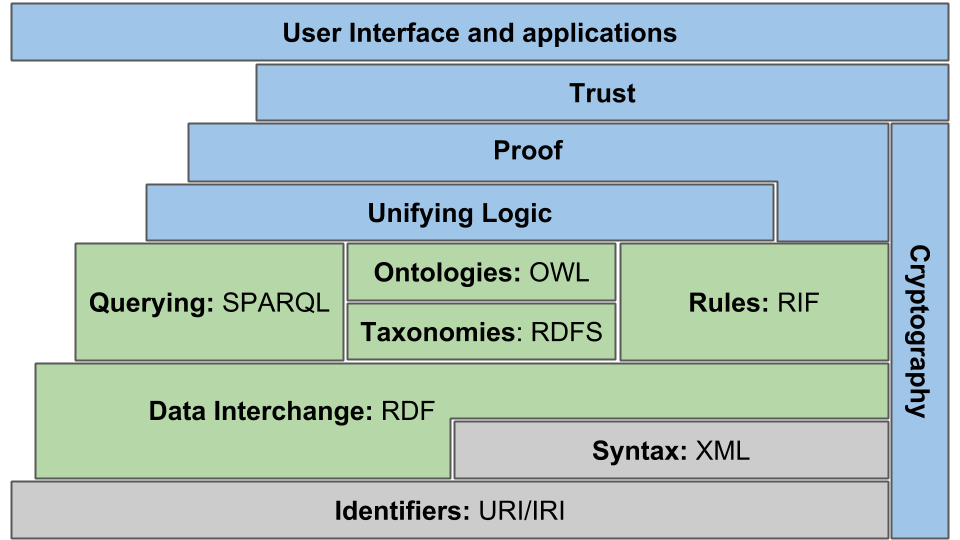
\includegraphics[width=0.8\textwidth]{stack6}
	%\end{adjustwidth}
	\caption[Semantic Web Stack]{Semantic Web Stack.}
	\label{fig:stack}
\end{figure}
%\footnotetext{Source: \url{https://en.wikipedia.org/wiki/Semantic_Web_Stack}}
Each layer placed on top of other layers  depends on  these other layers but not on those above them. Neighbouring layers can, but not necessarily have to make use of each other. 
We go from the bottom of the stack to its top to explain all its elements:

\begin{description}
%  \item[Character Set] To be compatible with the current Web and its applications, but also with textual documents in all languages in general,
%  the Semantic Web relies on Unicode.
 \item[Identifiers] The Semantic Web is a global network which relies on interoperability. In such a big setting, it is crucial that the names of individuals and concepts are unique.
 For their representation Uniform Resource Identifiers (\uris) and Internationalized Resource Identifiers (\iri{}s) are used.  
 \item[Syntax] There are several syntax formats frequently used in the Semantic Web. Standards of the World Wide Web are employed---such as XML or JSON---but also formats 
 only created for the Semantic Web such as for example the Terse RDF Triple Language (Turtle). 
%  The fact that the Semantic Web stack only mentions XML and omits 
%  other notations which are also used
%  is often 
%  a point of criticism.\footnote{See for example the discussion at: \url{https://lists.w3.org/Archives/Public/semantic-web/2016Feb/0121.html}.} 
 \item[Data Interchange]
In order to exchange data it must be agreed on  a common structure to express knowledge. This 
structure should not be too complex for a machine to parse but still 
powerful enough to make simple statements and connections. 
In the Semantic Web the Resource Description Framework (\rdf) was developed with 
that goal in mind. Knowledge is expressed using simple triples consisting of subject,
predicate and object. By using unique names (\iri{}s and \uris) connections between different triples are made. 
Ideally, one resulting graph then forms the Semantic Web.
 \item[Taxonomies] For the simple classification of objects and properties the Semantic Web uses the standard \rdf Schema (\rdf{}S). \rdf{}S extends the basic representation format 
 \rdf by several predicates with a predefined meaning such as for example \texttt{rdfs:subclassOf} to denote that one class is a subclass of another. 
 %
 \item[Ontologies]
 The taxonomy already gives some basic information about concepts and individuals in the web. To express more complex things in a fixed way, ontologies are used. 
 Ontologies can be understood as a collection of statements about concepts, classes and individuals using a broad variety of logical predicates which have a fixed meaning for the computer.
 Even though, in that sense a collection of rules over \rdf data could be understood as an ontology,  in the Semantic Web context the term refers to a set of statements written in the Web 
 Ontology Language (\owl). This language is based on description logics and a reasoner can use these statements to draw conclusions.
 %
 \item[Rules] Alternatively to \owl, but also in combination with this standard, there is another way of stating knowledge about concepts and data in the Semantic Web: rules. 
 Having their origin in classical logic programming, rules are used to directly state which triples or patterns of triples can be concluded from given information. To combine rule-based reasoning 
 with \owl reasoning the Semantic Web Rule Language (swrl) can be used. As a general format to exchange different kinds of rules, the Rule Interchange Format (RIF) was created. 
 There are also many other 
 rule-based logics used in the Semantic Web which are not standardised (yet), one of them is \notationthree Logic (\nthreelogic) 
 which is the subject of this thesis.
 %
 \item[Querying] Independently of whether reasoning is performed on \rdf data or not, there are many situations in which a user or an application wants to retrieve information 
 by searching for triples of a certain kind. Therefore, querying is an important part of the Semantic Web. To query data from \rdf the SPARQL Protocol And RDF Query Language (SPARQL) is used.
 \end{description}
 The different layers described so far have---at least up to some point---already been realised---for all building blocks there exist standards. 
 The higher layers we discuss now
are either not realised yet or the community has not yet agreed on a solution (or even on a concrete definition of the problem). 
% In that sense the  following description might be subjective. For alternative views we recommend for example 
% the introduction done by Hogan \cite{hogan}.
 \begin{description}
 \item[Unifying Logic]
 Above these concepts of querying, ontologies and rule based reasoning, there is the layer of a unifying logic: 
 a logical framework which connects the other concepts and makes it possible interoperate between them. 
The logic should thus support the inference mechanisms of these three underlying concepts and the formats below, in particular \rdf.
 \item[Proof]
 Once this unifying logic is found, it should be possible to provide formal proofs for the derivations done using this logic (and thereby also for all derivations of the underlying standards). 
 These proofs should be exchangeable by different parties and it should be possible to automatically check their correctness. Additional information like for example the source of knowledge 
 used could also form part
 of these proofs.
 \item[Cryptography]
 The cryptography layer lies aside of the layers discussed so far. For all the resources and at all layers of the Semantic Web cryptographic techniques should be used 
 to for example verify the identity of an agent or to implement access control mechanisms. Here, existing Web technologies and protocols like for example RSA or HTTPS but 
 also newer techniques like blockchain could be used.
 \item[Trust]
 The layers proof and cryptography together form the base for the trust layer: only if reasoning steps, sources of information and the trustworthiness of all parties involved
 can be verified and manipulation 
 can be excluded, people and machines can trust the information they get from the Semantic Web.
 \item[User interface and applications]
 This highest layer of the stack is also the broadest: a Semantic Web only makes sense if it is more than a scientific construct. 
 It needs to be used by humans but also by different machines which, following
 the original vision, should be able to interact between each other and make use of the resources available. Of course there are already applications making use of the Semantic Web implemented, but
 together with the progress of the Semantic Web as a whole, we expect a lot more to come.
\end{description}

%After having briefly introduced the Semantic Web Stack, it is worth to mention that there are different points which are 
% Introduction given by Hogan \cite{hogan}.
% Gerber \cite{Gerber} \cite{Gerber2}. Really nice: abstracts from technnologies. Bad: the word ``unifying Logic'' dissapeared.
% 
% Ian Horrocks: two towers \cite{twotowers} -- by supporting the closed world assumption we get two semantic webs.
% 
% 
% \cite{rearch} Paper by Boley, Kifer, etc. ``realistic'' architecture, not just one technology. 
% 
% 
% \subsection{Data Interchange}
% RDF
% 
% \cite{rdf}
% \subsection{Querying}
% \subsection{Ontologies}
% RDFS
% OWL
Introducing the Semantic Web stack, its critical points should also be discussed:

%Above, we explained, that the upper layers of the Semantic Web stack should depend on the lower ones, this particular detail often leads to discussion on several levels  

One problem which often leads to disputes\footnote{See for example: \url{https://lists.w3.org/Archives/Public/semantic-web/2016Feb/0121.html}} 
is that the current stack explicitly names XML~\cite{XML} as a base for the syntax while many applications rather use formats like 
the JSON-based JSON-LD~\cite{jsonld} or Turtle~\cite{turtle}, 
which is also easy to read for humans, to represent \rdf.\footnote{Even though in the case of Turtle this point 
is somehow addressed as the \rdf layer directly 
touches the layer of identifiers which are directly used by Turtle.} This is certainly a valid criticism. 
However, in this thesis we see the formats occurring in the stack as open lists of formalisms which have already been standardized to serve the purpose mentioned 
rather than a simple declaration of the decision in favour of a format. To emphasize this, we added to every layer which is labelled with a standard also the general purpose this layer 
fulfils. These names are not always present in the original stack our figure is based on.

Another detail of the stack which is often criticised has to do with the middle layer: While \owl and SPARQL are concrete logics---in case of \owl 
with sub-logics~\cite{OWLRL}---disposing 
over their own clearly defined unambiguous semantics (see \cite{owlrdfsem,owldsem} 
and \cite{sparql}, respectively), RIF~\cite{rif} is a format to interchange rules. Being designed for that purpose, RIF supports different paradigms with sometimes 
conflicting model-theoretic semantics (eg well-founded vs stable semantics) or even with no model-theoretic semantics at all: 
for the RIF Production Rule Dialect (RIF-PRD)~\cite{rifprd} only operational semantics is defined. 
As a connection between these formats, RIF offers RIF Core \cite{rifcore}, a minimal rule language supporting common features of rule languages which can be 
extended to define the semantics of concrete languages.
This broad support of different forms of rule-based languages makes it easy to create a new rule language and relate it to the standard---in that sense it is really
appealing from a theoretical point of view---but it also forms a burden for the bigger goal
behind the Semantic Web Stack: the realisation of the Semantic Web. Practitioners creating applications want to \emph{use rules}
and not  \emph{create or compare rule languages}. For the outsider the complex RIF landscape can be overwhelming. This is one possible reason why the 
full potential of RIF is barely used in practice. 

% Another aspect weakening the position of RIF in the stack is that its syntax is directly based on XML 
% and not on \rdf which offers different syntactic variants of which only one is \rdf/XML. 
% This makes the connection to \rdf rather loose

As discussed above, the upper layers of the Semantic Web stack should depend on the lower ones. 
Above, we already discussed that in the case of the syntax layer this is not always the case 
since XML is only one syntactical option to represent \rdf. The dependency problem is also given for the upper layers depending on \rdf:

RIF is independent of \rdf and poses own semantic definitions. The integration of \rdf into RIF can be done using so-called slots, an extra note~\cite{rifrdf} 
explains how RIF dialects 
can be semantically aligned with \rdf. 
%\rdf and \owl can be integrated to RIF via so-called slots, the   
%
%Nevertheless, even this group of 
%This means that it is a family of logics which do not all have Semantics defined.
%As it is, RIF is a very good format to \emph{define} languages, but with its oneness   
% Being a very open standard, RIF misses the opportunity to force the community to stick to a certain rule format which is crucial if we have in mind that it was created to 
% serve : the crea Semantic Web.
%RIF is standardised disagreement

SPARQL has its own query semantics which is agnostic about the meaning of \rdf triples. For SPARQL these are only patterns but these patterns need to be aligned 
with the search patterns of SPARQL.

More problematic is the relationship of \owl and \rdf. \owl  has been designed on the base of Description Logics~\cite{dl}. a logical framework based on First Order Logic 
which---in contrast to the latter---has the advantage to be decidable. For \owl there exist two syntaxes, one direct syntax 



In my opinion, only SPARQL is compatible with RDF (but I have to think about it) -> naja, sparql definiert nur query pattern und is in gewissen sinne agnostisch was die bedeutung der triple betrifft.

Here: Problems with Ontology layer

Even the parts realised have certain ``cracks'' or problems. It was mentioned earlier that all higher layers should rely
on the layers beneath them. That said, one would expect that \owl would be compatible with \rdf{}S---and there exists a version which actually is, \owl full. 

Must it even be \emph{one} unifying logic?

\section{The Unifying Logic}



Mention: RDF is only compatible with owl full

\cite{twotowers} think that the rules and owl should not be side by side, they see the open world assumption as problem and want to have the rule layer on top of owl dl.

Maybe also mention that the connection of owl and rdfs is rather artificial -> two semantic definitions...

%\subsection{Rule Based Logics}

History about big discussion open vs. closed world assumption.

Discussion: closed world assumption a problem

comes also in \cite{rearch}.

Solution:scoped negation as failure.

The paper above sees rules without negation as failure such as swrl just as extension of owl and not as belonging to the other format.

rules and owl see each other as black boxes.
we can combine them
-> this reminds me a little bit of validation where we first do dl reasoning and then querying

the paper also see querying as some kind of rule application (I think they are right here).


RIF

SWRL

N3

\cite{N3Logic}

Explain this unifying logic, list the attempts to find one and answer the question: why N3 and not those?



Here or somewhere else mention description logic programs \cite{DLP} which try to combine Description Logic and Logic Programming. - OK, rather their intersection.

\cite{knorr} rules as unifying logic

\cite{unilogic} first attempt to close the rift between rule-based and description logic reasoning, problem remains: open world assumption


What do we expect from the ``unifying logic''?

The vision of the Semantic Web is to enable machines to use the Web just as humans do. For that they need to be able to \emph{understand} and \emph{exchange} data through the Web. 
An unambiguous way to express knowledge is needed, a logic. 
This logic needs to be well defined to avoid misunderstandings and it needs to be agreed on this definition between all possible parties involved.


Different approaches in the ``quest for a unifying logic'': extend owl (nominal schemas, same paper \cite{unilogic}), ``merge'' owl and rules (both mentioned in \cite{unilogic}). We go a third way: rules for all.

approaches consider worst case time complexity (e.g. \cite{unilogic}). -> argue that this is nice but we focus on practical cases.

OWL and rdf is already artificial, rules are natural extension of RDF and the can cover owl.

Later on mention integrity constraints on data bases which are needed for validation.

Artikel von Motnik \cite{DLASP} sagt was ueber default rules for validation -> validation ist ein ziemlich interessantes Thema hier.

unifying logic on application level, not just a construct -> we therefore exclude owl full.

allgemein: answer set programming hat zwei Formen der Nagation.

noch was von Lifschitz und asp zitieren.


Also say why you should go for N3: unifying logic is not just a theoretical construct, it also gives practical advantages: reasoning is often faster when you use only one logic.  

somewhere: reification is not the same as citation.

Knorr hat DL style syntax
It has advantages if you need 
the features of different frameworks. Of course, if you know that, eg only querying is needed you should still go for SPARQL.


% The Unifying Logic needs to be well-defined in itself, it needs to be able to ``understand'' the underlying formats, in particular to query, do DL reasoning and use rules. 
% Additionally it should provide the opportunity to connect to the proof layer.
Requirements:
\begin{description}
 \item[clear semantic definition] 
The meaning of every statement needs to be clearly defined.
 \item[compatibility with existing Web standards]  Existing standards of the Semantic Web need to be supported. 
 In particular, querying, Description Logics, and rule based reasoning need to be covered.
 \item[support of proofs] It must be possible to express, interchange and check all derivations made in the logic.
 \item[capability to handle change] It must be possible to express and reason about change.
\end{description}



\section{Research questions}
Question: Is N3 a suitable candidate to become the unifying logic for the semantic web?

Sub-questions:

Can we give a clear semantic definition of Notation3 Logic?

How does Notation3 Logic interfere with other formats? Can SPARQL, OWL and RIF be expressed?

Is it possible to express proofs in N3?

Can N3 handle change?

I think I need to be more specific. To find that: what do I actually do here?



% \textbf{Part 4: going beyond the limits}
% 
% introduce weighted transition logic to express change
% 
% This part is optional



Somewhere I need to talk about problems, especially decidability and for example the problems of OWL full.

Should I have a chapter about negation as failure?

Problem: blank nodes in SPARQL

\part{Semantics}\label{semantics}

\chapter{Motivation and Problems}\label{problem}
use mention problem
%
\section{Syntax}
Before coming to the main topic of this paper, implicit quantification, we start by defining the general syntax of N3Logic. We exclude built-ins %, as their 
%meaning is mostly defined on the corresponding website, %\footnote{See \url{http://www.w3.org/2000/10/swap/doc/cwmBuiltins}.},  
and explicit quantification (for more information see section \ref{expl}). %\footnote{We explain this choice in section \ref{expl}. }. 
%The latter is, as well as its implicit counterpart, not trivial. We will give a quick explanation of that at the end of this paper.\\
The syntax-definition below is oriented on the context-free grammar as provided at the team submission web page \cite{Notation3}. 
%We limit our developments to the %, at least in our opinion, 
%most important properties of \nthree---quantification, implication and quoting---and skip most inbuilt-predicates of \nthree and \rdf, whose meaning 
%can be found on the corresponding websites. %We start with the vocabulary:


\begin{definition}[Basic N3 vocabulary]\label{voc}
An \emph{N3 alphabet~$A$} consists of the following disjoint classes of symbols:
\begin{itemize}
\item A set $U$ of \uri symbols.
\item A set $V=V_E\mathbin{\dot{\cup}} V_U$  of (quantified) variables, with $V_E$ being the set of existential variables
and $V_U$ the set of universal variables.
\item A set $L$  of literals.
%\item A boolean literal \verb!false!
\item Brackets \verb!{!, \verb!}!, \verb!(!, \verb!)!
\item Logical implication $\verb!=>!$ 
\item Period \verb!.!
\end{itemize}
\end{definition}

%We define the elements of $U$ in the same way as \rdf \cite{rdf}. %in %the corresponding specification~\cite{iri}.
%Like Turtle, \nthree allows to abbreviate URLs as prefixed names~\cite{turtle}.
%Literals are strings beginning and ending with quotation marks `\verb!"!';
%existentials start with `\verb!_:!', universals with `\verb!?!'.\\
%As \nthree does not clearly distinguish between predicates and constants---a single \uri symbol can stand for both at the same time---we have to change the first-order-concept of a 
%term to something similar:

We define the elements of $U$ as in the corresponding specification~\cite{iri}. As for example in Turtle \cite{turtle},
\nthree allows  to abbreviate URLs by using prefixes.
%\nthree allows to abbreviate URLs as prefixed names~\cite{turtle}.
Literals are strings beginning and ending with quotation marks `\verb!"!';
existentials start with `\verb!_:!', universals with `\verb!?!'.
%
Unlike first order logic, \nthree does not distinguish between predicates and constants---%
a single \uri symbol can stand for both at the same time---%
so the first-order-concept of a~\emph{term}
has a~slightly different counterpart in \nthree: an \emph{expression}.
Since the definition of expressions (Definition~\ref{expression})
is closely related to the concept of a~formula (Definition~\ref{formula}),
the two following definitions should be considered together.

%We include the possibility of quoting formulas by introducing \emph{formula expressions}. Additionally to the direct citation of a formula, there are two other 
%kinds of formula-expressions: the empty expression (true) and \verb!false!. As the latter is inherited from \rdf, it can't be understood as a formula itself as the 
%similar expression in first order logic normally is. The declarations as formula expressions enable us to keep that kind of meaning in controlled situations, as will
%be shown in the following chapters.


\begin{definition}[Expressions]\label{expression}
  Let $A$ be an \nthree alphabet.
  The set of \textit{expressions} $E \subset A^{*}$ is
  defined as follows:
  \begin{enumerate}
    \item Each \uri is an expression.
    \item Each variable is an expression.
    \item Each literal is an expression.
    \item \label{list} If $e_1,\ldots,e_n$ are expressions, $\verb!(!e_1 \ldots e_n\verb!)!$ is an expression. 
    %\item \label{false} \verb!false! is an expression.
   % \item $\verb!{ }!$ is an expression.
    \item \label{fe} If $f\in F$ is a formula, then $\verb!{!f\verb!}!$ is an expression. 
  \end{enumerate}
  The expression defined by \ref{list} is called a \textit{list}.
  We call the expressions defined by %\ref{false}--
  \ref{fe}
  \textit{formula expressions} and denote the set of all formula expressions by $\mbox{\textit{FE}}$.
\end{definition}


Note that point \ref{fe} of the definition above makes use of formulas, which are defined as follows:

\begin{definition}[\nthree Formulas]
    \label{formula}
    The set $F$ of \textit{\nthree formulas} over an alphabet $A$ is recursively defined as follows:
    \begin{enumerate}  
      \item \label{1} If $e_1, e_2, e_3$ are expressions, $e_1~ e_2~ e_3$. is a formula, an \textit{atomic} formula.
      \item \label{2} If $t_1, t_2$ are formula expressions, $t_{1} \verb!=>!~t_{2}.$ is a formula, an \textit{implication}.
      \item \label{n} If $f_1$ and $f_2$ are formulas, $f_1 f_2$ is a formula, a \textit{conjunction}.
    \end{enumerate}
\end{definition}

We will refer to a~formula without any variables as a~\textit{ground formula}.
Analogously, we call such kind of expressions \textit{ground expressions}.
We denote the corresponding sets by $F_g$ respectively $E_g$.\\
%Note that 
%Althouh we see this rarely used in practice, t
The definition explicitly allows all expressions in all positions of atomic formulas. 
Literals or even formula expressions can be subjects, objects or predicates.

%Whether a triple with a 
%
%It is rather unlikely th
%It is rather unlikely that any
%Whether an element 
%The meaning of those expressions depends on the respective interpretation.

%We will refer to a~formula without any variables as a~\textit{ground formula}.
%Analogously, we call expressions without any variables \textit{ground expressions}.
%We denote the corresponding sets by $F_g$ respectively $E_g$.
% We are going to define the semantics of a formula. To enable the reader to distinguish between mathematical symbols describing the language and \nthree-constructs (expressions and formulas), 
% we mark the latter by underlinement. 

In the examples in the remainder of this paper, we will use the common \rdf shortcuts:

\begin{remark}[Syntactic variants]\label{rem}
\begin{itemize}
\item A formula consisting of two triple subformulas starting with the same element \verb!<d> <p> <e>. <d> <q> <f>.! can be abbreviated using a semicolon:\newline 
\verb!<d> <p> <e>; <q> <f>.!
\item Two triple formulas sharing the first two elements  \verb!<d> <p> <e>. <d> <p> <f>.! can be abbreviated using a comma: \verb!<d> <p> <e>, <f>.!
%  \item \verb![]! can be used as an expression and is a shortcut for a new existential variable. So \verb![] <p> <d>.! stands for \verb!_:x <p> <d>.!
%  If $[~]$ occurs in a formula $f$ instead of an expression, each instance of $[~]$  can be translated by a new existential variable.
 \item An expression of the form \verb![<p> <o>]! is a shortcut for a new existential variable \verb!_:x!,
   which is subject to the statement \verb!_:x <p> <o>.! %\linebreak
   So \verb! <s> <p> [<q> <o>].! stands for \verb!<s> <p> _:x. _:x <q> <o>.!
 %\item \verb!a! is a~shortcut for \verb!rdf:type!~\cite{RDF}.
 \end{itemize}
\end{remark}



To emphasize the difference between brackets which form part of the \nthree vocabulary, i.e. ``\verb!(!'', ``\verb!)!'', ``\verb!{!'', and ``\verb!}!'', 
and the brackets occurring in mathematical language, we will underline the \nthree brackets in all definitions where both kinds of brackets occur.

%\section{Quantification}\label{quantsec}
%The examples of implicit quantification given in Section~\ref{n3examples} were rather  
The example formulas we discussed in Section~\ref{n3examples} were rather simple and understanding their intended meaning was not 
 difficult (maybe with the exception of cited formulas which can lead to discussions \cite{TriGsemantics}). For the only case where 
two different interpretations were plausible -- Formula~\ref{both} which had universals and existentials occurring together --
the \wwwc team submission~\cite{Notation3} contains a clear statement which interpretation needs to be chosen: \\
% This is different when it comes to implicit quantification. Just like \rdf, \nthree allows the 
% The examples of \nthree formulas given so far were rather easy and their interpretation was rather straightforward
% (maybe with the exception of cited formulas which can lead to discussions \cite{TriGsemantics}).
% This is different when it comes to implicit quantification. Just like \rdf, \nthree allows the usage of implicitly existentially quantified variables, called \emph{blank nodes}.
% Blank nodes either start with ``\verb!_:!'' or are expressed using square brackets ``\texttt{[~]}''. 

\MyQuote{ \label{beide} ``If both universal and existential quantification are specified for the same formula, 
then the scope of the universal quantification is outside the scope of the existentials''.}

Unfortunately, not all cases are that clear.
% 
% 
% in Section~\ref{n3examples}, we gave a few examples for \nthree formulas and their intended meanings. Since \nthree aims to extend \rdf, a \wwwc standard with well-defined 
% semantics, the meaning of simple  
%
% In the cases illustrated in Section~\ref{n3examples}, the interpretation of the implicitly quantified formulas was rather easy:
% the variables are existentially and universally quantified at the top of the formula; 
% if they co-occur in the same formula, the universal quantification dominates the existential. 
When implicitly quantified variables occur in deeply nested formulas, 
 their intended meaning is not always obvious and the interpretations of such formulas sometimes differ between reasoning engines. 
%
%In the next subsections we give examples for such ambiguous formulas.
In this section we want to better understand these differences. 
With this goal, we perform several tests on the reasoners Cwm \cite{cwm} and EYE~\cite{eyepaper} and compare their results. 
Cwm and EYE were chosen because they cover most constructs specified in \nthree{}'s \wwwc team submission. 
In contrast to for example FuXi~\cite{fuxi}, they both support rather complex constructs like nested rules. 
% and because they differ in their way to handle 
% implicit universal quantification.
% Further details about how differences can be detected can be found in our previous paper \cite{arndt_ruleml_2015}. % and in \ref{ap1}.



% 
% Before clarifying syntax and semantics of \nthree in a more formal way than presented in Section~\ref{n3examples}, 
% we test how implicit quantification of \nthreelogic is understood in practice. We  take a look to the official sources of \nthree, namely the \wwwc team submission~\cite{Notation3}
% and the journal paper about \nthree~\cite{N3Logic}, and test, how the reasoners Cwm~\cite{cwm} and EYE~\cite{eye} understand them. 
% We choose these two reasoners because of their coverage: while for example FuXi~\cite{fuxi} only supports \nthree datalog -- a subset of \nthree which does not support nested rules --
% the reasoners Cwm and EYE cover a big part of the specifications
% As in \rdf, atomic formulas are triples consisting of subject, predicate and object. They can be intuitively understood as 
% first order formulas of the form \linebreak $\text{predicate}(\text{subject}, \text{object})$. It is also easy to get an idea of the meaning of conjunctions or implications 
% if no variables are involved. Including implicit quantification is more difficult.
% Definition \ref{voc} distinguishes between two kinds of variables: universal and existential variables. 
% As the names indicate, these variables are meant to be implicitly quantified. But how do we have to understand this ``implicit'' quantification?
% Some cases are quite simple. 
% If we have the formulas
% \[
% \verb! _:x :knows :Kurt.! \text{ and } \verb! ?x :knows :Kurt.!
% \]
% It is rather straight forward to understand them as ``someone knows Kurt.'' and ``everyone knows Kurt.'' In first order logic:
% %We can understand that as the fact that Kurt knows someone or something, written in first order logic:
% \[
% \exists x: \text{knows}(x, \text{Kurt}) \text{ and } \forall x: \text{knows}(x, \text{Kurt}).
% \]
%Similarly simple constructions with universals can be understood:
%\[
%\verb! ?x :knows :Kurt.!
%\]
%Means that everyone knows Kurt, in first order:
%\[
%\forall x: \text{knows}(x, \text{Kurt}).
%\]
% But the above grammar also enables us to construct more complicate statements. Does the construct 
% \begin{equation}\label{both} \verb! ?x :loves _:y.!\end{equation} mean 
% ``everybody loves someone'' or ``there is someone
% who is loved by everyone'', in first order formulas: 
% %\[\forall x \exists y : \text{loves}(x,y) \tag{1}\quad \text{ vs. } \exists y \forall x : \text{loves}(x,y)\]
% \stepcounter{equation}
% \begin{equation} % oder auch align
% \forall x \exists y : \text{loves}(x,y)\quad  \text{ vs. }\quad \exists y \forall x : \text{loves}(x,y) \tag{\ref{both}a, b}
% \end{equation}
% 
% 
% In this case we know the answer, the team submission \cite{Notation3} clearly chooses (\ref{both}a): 
% 
% \MyQuote{ \label{beide} ``If both universal and existential quantification are specified for the same formula, 
% then the scope of the universal quantification is outside the scope of the existentials''.}
% %
% And also the reasoners we tested, in particular EYE and cwm, have implemented the first interpretation (\ref{both}a).
% %\\
% 
% Such clarity is lacking when it comes to nested formulas or co-occurring formula expressions which contain variables. 
% We will treat this in the following sections, first for existential variables, then for universals.
%This is the topic of the following sections.

\subsection{Existentials}\label{existentials}
We start our considerations by taking a closer look to implicit existential quantification in nested formulas, 
ie formulas where the blank node occurs within curly brackets \{~\}.  Such constructs are typically used to cite formulas or
to state rules. We take the following example for the latter:
%An example for such a formula is the following:
% 
% To test how both cwm and EYE understand existential quantification, we confronted them with some examples.
% Both reasoners offer the option to output all knowledge they are aware of, this includes all derived formulas and rules as well as the
% input. In most cases, different variables sharing the same name are renamed to be distinguishable. %standardized apart\footnote{Cwm does standardization apart for existentials, 
% %using square brackets ``\texttt{[ ]}'' as introduced in Remark \ref{rem}, EYE employs Prolog's standardization apart.}. %, in EYE this process includes standardization apart\footnote{As EYE is written in Prolog, 
% %Prolog's standardization apart mechanism is used see e.g. CITATION}.   
% Therefore we can use the derived output of such a reasoning process with a simple rule as input as indication of
% how the formula is interpreted. As a first example %for our tests we took 
% we invoked both reasoners with
% a formula with nested existentials:
\begin{equation}\label{eq1}
\verb!_:x :says {_:x :knows :Albert.}.!
 \end{equation}
%  \begin{equation}\label{eqrule}
% \verb!{_:x :knows :Albert.}=>{:Albert :knows _:x.}.!
%  \end{equation}
This triple is interesting because it contains the blank node \texttt{\_:x} at two positions: as a subject of the triple and inside a nested formula. We already know 
that a blank node represents an implicitly existentially quantified variable, but what we do not know yet is: what is the exact position of its quantifier 
and what is the scope of the variable? Depending on the answer, the two occurrences of \texttt{\_:x} could either refer to the same instance of the domain of discourse, 
then the formula means
%The formula could either mean
%
\[\exists x : \text{says}(x, \text{knows}(x, \text{Albert})) \tag{\ref{eq1}a} \label{zwei}\]
\begin{center}\textit{``There exists someone who says about himself that he knows Albert.''}
  \end{center}
  or 
%   it can refer to two (possibly) different individuals. Here, we have two options:
    the \texttt{\_:x} is always quantified in the direct formula it occurs in (ie the brackets \texttt{\{~\}}), then the two existentials can refer to different objects 
  and we get
%  
% \[
% \exists x_1 : \exists x_2: \text{says}(x_1, ( \text{knows}(x_2, \text{Albert})))\tag{\ref{eq1}b} \label{zw1}\]
% \begin{center}\textit{``There exists some $x_1$ and some $x_2$ and  $x_1$ says about $x_2$ that he knows Albert.''}\end{center}
\[
\exists x_1 : \text{says}(x_1, (\exists x_2: \text{knows}(x_2, \text{Albert})))\tag{\ref{eq1}b} \label{zw}\]
\begin{center}\textit{``There exists someone who says that there exists someone (possibly someone else) who knows Albert.''}\end{center}
\begin{lstlisting}[
  float=t,
  caption={Reasoning result of cwm for Formula \ref{eq1}. The two occurrences of the variable \texttt{\_:x} get translated to two blank nodes in square bracket notation. },
  label=cwm1]
§\textcolor{gray}{@prefix : <http://example.org/ex\#>.}§

[ :says { [ :knows :Albert ]. } ].
\end{lstlisting}

\begin{lstlisting}[
  float=t,
  caption={Reasoning result of EYE for Formula \ref{eq1}. The two occurrences of the variable \texttt{\_:x} get translated to two different blank nodes.},
  label=third]
§\textcolor{gray}{PREFIX : <http://example.org/ex\#>}§

_:t_0 :says {_:t_1 :knows :Albert}.
\end{lstlisting}
As explained earlier in Section~\ref{prn3}, \nthree reasoners can be invoked to output the deductive closure of their input files. If we provide 
Cwm and EYE with Formula~\ref{eq1}  and let them derive the deductive closure we get the result displayed in Listings~\ref{cwm1} and \ref{third}, respectively.\footnote{
Unless indicated otherwise we use in this thesis the following versions of the reasoners:
Cwm v 1.197 2007/12/13 15:38:39 syosi and EYE v18.0312.0936}
We see, that Cwm uses the bracket notation \texttt{[~]}  for blank nodes where, as explained in Section~\ref{vars}, every new bracket refers to a fresh new blank node; 
EYE gives them different names (\texttt{\_:t\_1} and \texttt{\_:t\_2}). This behaviour shows, that both reasoners understand the two occurrences of \texttt{\_:x} as different 
blank nodes which results in Interpretation~\ref{zw}.%
\footnote{
Strictly speaking, this example still does not make sure that the reasoners really assume Interpretation~\ref{zw} since both blank nodes could be quantified on top level:
$\exists x_1 : \exists x_2: \text{says}(x_1, ( \text{knows}(x_2, \text{Albert})))$.
To exclude this possibility the reasoners can be tested with Triple~\ref{simple} and the rule \texttt{\{\_:x :knows :Albert.\} => \{:Albert :is :known.\}.}: only if 
the quantifier for the blank node is in the antecedent of the rule, this input results in \texttt{:Albert :is :known.} This is the case for both reasoners.
}
%but we do not know from that example, whether this separation really results in Interpretation~\ref{zw}. It could still be that the reasoners understand the quantifier

% Strictly speaking, this example still does not make sure that the reasoners really assume Interpretation~\ref{zw} since the quantifiers for the blank nodes in the formulas are 
% not written down and the formula could still have the following meaning:
% \[
% \exists x_1 : \exists x_2: \text{says}(x_1, ( \text{knows}(x_2, \text{Albert})))\tag{\ref{eq1}c} \label{zw1}\]
% \begin{center}\textit{``There exists some $x_1$ and some $x_2$ and  $x_1$ says about $x_2$ that he knows Albert.''}\end{center}
% To exclude this possibility, we do one extra test. Depending on the position of the existential quantifier the rule 
% % Is there someone who says about himself that he knows Albert, or does this someone just state that someone exists who knows Albert?
% % In first order logic
% % \[\exists x : \text{says}(x, \text{knows}(x, \text{Albert})) \tag{\ref{eq1}a}\]
% % \hspace{6cm} or
% % \[\exists x_1 : \text{says}(x_1, (\exists x_2: \text{knows}(x_2, \text{Albert})))\tag{\ref{eq1}b} \label{zwei}\]
% % %
% % Listing \ref{third} shows the output of EYE given formula (\ref{eq1}) as only input, Listing \ref{cwm1} the output of cwm. 
% % We clearly see\footnote{To see this evidence 
% % for cwm, recall that every new bracket ``\texttt{[}$\ldots$\texttt{]}'' corresponds with a \emph{new} existential variable, see also Remark \ref{rem} or \cite{turtle} for further information. }
% % that both reasoners favor 
% % option (\ref{zwei}).  
% 
% 
% 
% %\footenotetext
% 
% %\FloatBarrier
% % 
% % 
% % We observe similar behavior using the same existential quantifier in two co-occurring graphs.
% % In an example formula such as 
% %
% \begin{equation} \label{ruru}
% \verb!{_:x :knows :Albert.} => {:Albert :is :known.}.! 
% \end{equation}
% either translates to
% \[
% (\exists x: \text{knows}(x,\text{Albert}))\rightarrow \text{is}(\text{Albert}, \text{known})\tag{\ref{ruru}a}
% \]
% in which case the formula is equivalent to 
% \[
% \forall x:( \text{knows}(x,\text{Albert}))\rightarrow \text{is}(\text{Albert}, \text{known})\tag{\ref{ruru}a'}
% \]
% or it translates to
% \[
% \exists x:( \text{knows}(x,\text{Albert}))\rightarrow \text{is}(\text{Albert}, \text{known})\tag{\ref{ruru}b}
% \]
% These two options can be tested against each other by giving Rule~\ref{ruru} to the reasoners together with Triple~\ref{simple},
% $\verb! :Kurt :knows :Albert.!
% $, if the reasoners derive 
% \begin{equation}
%  \verb!:Albert :is :known.!
% \end{equation}
% we can assume that they favour 
% 
% 
% %So, for EYE, the scope of existential quantification is always only the direct formula expression the existential occurs in but 
% %not it nested dependencies.
% The two \verb!_:x! are interpreted as different variables by both reasoners. In first order logic this would be:
% \[
%  (\exists x_1: \text{knows}(x_1, \text{Albert}))\rightarrow (\exists x_2: \text{knows}(x_2, \text{Kurt}))
% \]
%
%
%
This example shows what is meant by the following quote from the \wwwc team submission \cite{Notation3}:

\MyQuote{
``When formulae are nested, \_: blank nodes syntax \emph{[is]} used 
to only identify blank node in the formula it occurs directly in. 
It is an arbitrary temporary name for a symbol which is existentially quantified within the current 
formula (not the whole file). They can only be used within a single formula, and not within nested formulae.''
}
%
%This means, the scope of an existential quantifier is always only the formula-expression ``\verb!{!$\ldots$\verb!}!'' it occurs in, but not its nested dependency.
%We added these two examples to be able to compare the interpretation of existential quantification with universal quantification.
%Although this section might not seem surprising, we included the above 
%We keep these examples for the scoping of existentials in the paper, to be able to emphasize the different scopes of existential and universal quantification.
In other words: existential variables are always quantified in the direct formula -- marked by curly brackets \texttt{\{~\}} -- they occur in. 
This quantifier does always only count for that formula and not for the nested formulas depending on it.


\subsection{Universals}\label{universals}
The case of implicit existential quantification in \nthree was still clear and the reasoners we tested did not disagree on the meaning of implicitly existentially 
quantified variables. This is different for universal quantification. A typical example for a formula containing universal quantification was given before in Formula~\ref{uni}:
\begin{multline}\tag{\ref{uni}}
 \texttt{\{:Kurt :knows ?x.\} => }%} \\ \texttt{
 \texttt{\{?x :knows :Kurt.\}.}%\nonumber
\end{multline}
It would not be very useful to handle the quantification in this equally as existential quantification. If universal quantifiers where also always quantified on their direct 
formula we would get the interpretation:
\[\tag{\ref{uni}a}
(\forall x_1: \text{knows}(\text{Kurt}, x_1))\rightarrow (\forall x_2: \text{knows}(x_2, \text{Kurt}))
\]
\begin{center}\textit{``If everyone knows Kurt then Kurt knows everyone''}
  \end{center}
Here, we would never be able to write any rules which reason on \rdf triples since this rule only gets invoked for a universal statement -- ``\textit{Everyone knows Kurt.}'' 
--  but it is not possible to 
make universal statements in plain \rdf. Therefore, the interpretation we already discussed earlier in Section~\ref{vars} is correct in this case:
\[\tag{\ref{uni}b}
\forall x:(\text{knows}(\text{Kurt}, x))\rightarrow (\text{knows}(x, \text{Kurt}))
\]
\begin{center}\textit{``Everyone Kurt knows also knows Kurt.''}
  \end{center}
The quantifier for both occurrences of \texttt{?x} is in front of the whole formula. But what happens if the universal variable occurs in a deeper nested formula? 
% We test 
% that on the following example:
% 
% 
%
Here,
the \wwwc team submission states the following:\\

\MyQuote{
 ``There is a also a shorthand syntax ?x which [...] implies that x is universally quantified not in the formula but in its \textbf{parent formula}.''}
We learn that universal variables are quantified on their \emph{parent formula}. Unfortunately neither the \wwwc team submission nor the journal paper about \nthreelogic 
provide us with a definition of that concept. We therefore perform some tests to better understand which formula is the parent.
 
Consider the following formula:
%When it comes to the definition of the scope, universal quantifiers are more complicated. To illustrate that, we consider the following example:
%Another example is the following formula:
%\\ %s and this is also how it is implemented in the reasoners we are considering in this paper, cwm and EYE. 
%It gets even more difficult when it comes to nested rules. As the critical example for this paper, we consider the formula 
\begin{multline}
\texttt{\{\{?x :p :a.\} => \{?x :q :b.\}.\} =>}\\
\texttt{\{\{?x :r :c.\} => \{?x :s :d.\}.\}.} \label{eq2} \end{multline}
Are all \verb!?x! the same? If not, which ones do we have to understand as equal and where are they quantified? 
Of the several options to interpret this formula, two seem to be most likely:
\[\forall x: ((p(x,a)\rightarrow q(x,b))\rightarrow ( r(x,c) \rightarrow s(x,d)))\tag{\ref{eq2}a}\label{ei}\]
\begin{center}or\end{center}
\vspace{-\baselineskip}
\begin{multline}
(\forall x_1: p(x_1,a)\rightarrow q(x_1,b))\rightarrow (\forall x_2: r(x_2,c) \rightarrow s(x_2,d))\tag{\ref{eq2}b}\label{ci}
\end{multline}
%But which interpretation is correct?
% \[
% (\forall x_1: p(x_1,a)\rightarrow q(x_1,b))\rightarrow (\forall x_2: r(x_2,c) \rightarrow s(x_2,d))\tag{\ref{eq2}a}
% \]
% \hspace{6cm}or
% \[\forall x: ((p(x,a)\rightarrow q(x,b))\rightarrow ( r(x,c) \rightarrow s(x,d)))\tag{\ref{eq2}b}\]
%In interpretation \ref{ci}, 
Interpretation~\ref{ei} understands the top formula as the parent of all other formulas, the quantifier for all occurrences of \texttt{?x} is on that formula.
For Interpretation~\ref{ci} the parent of the first two occurrences of \texttt{?x} is the formula 
\begin{equation}
\texttt{\{?x :p :a.\} => \{?x :q :b.\}.}\label{sub1}
\end{equation}
and the parent of the third and fourth occurrence of \texttt{?x} is the formula
\begin{equation}\texttt{\{?x :r :c.\} => \{?x :s :d.\}.}\label{sub2}\end{equation}
Therefore, these formulas carry quantifiers.

If a reasoner follows Interpretation~\ref{ei}, Formula~\ref{eq2} applied on the following rule
\begin{equation}\label{ss1}
 \texttt{\{:e :p :a.\} => \{:e :q :b.\}.}
\end{equation}
results in
\begin{equation}\texttt{\{:e :r :c.\} => \{:e :s :d.\}.}\label{ss2}\end{equation}
While this result cannot be derived by following Interpretation~\ref{ci}. %However, the latter yields Formula~\ref{sub2} when provided with Formula~\ref{sub1}.


If we test the reasoners Cwm and EYE with Formulas~\ref{eq2} and \ref{sub1} as input we get the results displayed in Listing~\ref{cwm2},\footnote{The 
predicate \texttt{log:implies} present in the original output is replaced here by implication arrow \texttt{=>}. The two symbols have the same meaning.} \ref{forth}, respectively.
\begin{lstlisting}[
  float=t,
  caption={Output of cwm for for Formulas~\ref{eq2} and \ref{ss1}. The reasoner does not derive Formula~\ref{ss2}. },
  label=cwm2]  
§\textcolor{gray}{@prefix : <http://example.org/ex\#>.}§
§\textcolor{gray}{   @prefix unive: <\#> .}§
{:e :p :a.}  => {:e :q :b .}.

{@forAll unive:x . {unive:x :p :a .}=>{unive:x :q :b.}.} 
=> 
{@forAll unive:x . {unive:x :r :c .}=>{unive:x :s :d .}.}.
\end{lstlisting}
\begin{lstlisting}[
  float=t,
  caption={Output of EYE for Formulas~\ref{eq2} and \ref{ss1}. The reasoner derives Formula~\ref{ss2}.  },
  label=forth]  
§\textcolor{gray}{PREFIX : <http://example.org/ex\#>}§

{{?U_0 :p :a}=>{?U_0 :q :b}}=>{{?U_0 :r :c}=>{?U_0 :s :d}}.
{:e :p :a} => {:e :q :b}.
{:e :r :c} => {:e :s :d}.
\end{lstlisting}
% The universals in the antecedent and consequent of the main implication reside in two different scopes.
% %This reflects Cwm's interpretation. % as two subformulas:
% Here, it is important that Formula~\ref{eq2} is composed of the subformulas:
% \begin{equation}
% \texttt{\{?x :p :a.\} => \{?x :q :b.\}.}\label{sub1}
% \end{equation}
% \begin{center}  
% and 
% \end{center}
% \begin{equation}\texttt{\{?x :r :c.\} => \{?x :s :d.\}.}\label{sub2}\end{equation} %are direct sub-formulas of formula \ref{eq22}. 
% Syntactically this division is marked by the use of curly brackets \texttt{\{\}}.
% Formula \ref{sub1} has two direct subformulas (again marked by brackets), namely:
% \[\texttt{\{?x :p :a.\}} \text{\hspace{0.5cm} and \hspace{0.5cm}} \texttt{\{?x :q :b.\}}\tag \label{\ref{sub1}a,b}\] 
% while
% \[\texttt{\{?x :r :c.\}} 
% \text{\hspace{0.5cm} and \hspace{0.5cm}} \texttt{\{?x :s :d.\}}
% \tag \label{\ref{sub2}a,b}\]are subformulas of Formula \ref{sub2}. 
%While it is rather easy to understand, how implicitly quantified universals are handled in EYE---they are all universally quantified on top level---it is
%worth to take a closer look into the quantification performed by cwm. 
% Cwm now applies the \wwwc team submission:
% 
% 
% \MyQuote{
%  ``There is a also a shorthand syntax ?x which [...] implies that x is universally quantified not in the formula but in its parent formula.''}
% %
We clearly see that Formula~\ref{ss2} is derived by EYE but not by Cwm. 
We furthermore see that the output of Cwm contains the key word \texttt{@forAll} at in beginning of the antecedent and of the consequent of the main rule in Lines 5 and 7. 
Here, this keyword has the same meaning as the first order symbol $\forall$. Cwm follows Interpretation~\ref{ci}.  We see that 
Cwm and EYE understand the concept of a \emph{parent} differently.
For the remainder of this thesis we write $\textit{parent}_c$ when we refer to the parent formula as implemented in Cwm and $\textit{parent}_e$ 
for the concept of a parent realised in EYE.

The previous example reveals a general problem: 
We needed to explain how the \wwwc team submission is \emph{interpreted} by the reasoners EYE and Cwm.
Of course the term \emph{parent formula} could be understood differently 
and only
specific testing made us come to our conclusion that the above are EYE's and Cwm's interpretations. % of the formula.
Most users are not even aware of the differences in interpretations and the lack of a formalism renders it difficult to discuss or even just express them. %---%
To come to a~clear and unambiguous definition of the logic, 
\nthree needs to be formalised and there needs to be a formalism to express the differences of existing interpretations. 
%This way, user can at least know how the
% The term \emph{parent formula} of a formula $f$ is understood as the next formula $g$ either occurring in curly brackets $\{g\}$ or being the top formula 
% for which $\texttt{\{}f\texttt{\}}$ is a direct component. % of the formula itself or -- in case it is a conjunction -- of one of its conjuncts.
% In our example, Formula~\ref{sub1} is the parent formula of Formulas~\ref{sub1}a and b, and Formula~\ref{sub2} is the parent formula of Formulas~\ref{sub2}a and b.
% This explains the scoping in interpretation \ref{ci}. We refer to this understanding of the concept  parent by using the subscript c, we write $\textit{parent}_c$.
% 
% This is the interpretation EYE applies. For the remainder of this paper we refer to this concept of the term by adding the subscript e, ie $\textit{parent}_e$ 
% refers 
% to the parent formula understood as the top formula.
% 
% 
% 
% 
% As above, we gave formula (\ref{eq2}) as input for both reasoners, cwm and EYE. 
% 
% Lines 1-9 of Listing \ref{forth} show the result of EYE which seems to imply\footnote{Where applicable, 
% EYE employs the ``standardization apart'' mechanism of its programming language Prolog.} that EYE supports the second interpretation (\ref{eq2}b), 
% but as it does not differ from the input, 
% we ran another test to verify that and added the formula 
% \begin{equation}\label{eq4} \verb!{:e :p :a.} => {:e :q :b.}.! \end{equation}
% to the reasoning input in order to see whether the reasoner outputs %(\ref{eq2}b) the reasoner's the result should contain the derived formula  
% \begin{equation}\verb!{:e :r :c.} => {:e :s :d.}.!\end{equation}
% as it would be the case with interpretation (\ref{eq2}b) but not with interpretation (\ref{eq2}a). % this formula cannot be derived. 
% The reasoning output of EYE shown in Listing \ref{forth} (all lines)
% verifies
% that EYE interprets all variables with the same name which occur in one single implication equally regardless of how deeply nested they occur. %variables with the same name in all nested formulas  equally within one single implication.
% 
% In contrast to this, Listing \ref{cwm2} shows the result cwm gives.  Here, the keyword\linebreak %\footnote{ For further explanation of the 
% %keyword \texttt{@forAll} see section \ref{expl}.} 
% ``\verb!@forAll!''
% can be understood as its first order counterpart ``$\forall$'' (see Section \ref{expl}). %Here we see a clear difference between that cwm's interpretation of the input differs from EYE. 
% Cwm understands 
% formula (\ref{eq2}) as stated in interpretation (\ref{eq2}a). Here we see a clear difference between the two reasoners.
% 
% 
% %\FloatBarrier
% 
% 
% After examining universals in co-ordinated expressions such as in the above implication, 
% we are also interested in how those variables are handled in subordinated formula expressions, similar to those in formula (\ref{eq1}). 
% We consider the following formula: 
% \begin{equation}\label{nest}
%  \verb!{?x :p :o.} => {?x :pp {?x :ppp :ooo.}.}.!
% \end{equation}
% To learn how the reasoners interpret this formula, we give the simple formula \begin{equation}\label{spo}\verb!:s :p :o.! \end{equation} as additional input. 
% Listings \ref{eye4} and \ref{cwm4} show the reasoning results of EYE respectively cwm. We clearly see that the two reasoners agree in their interpretation 
% and that this interpretation of formula (\ref{nest}) differs from the interpretation of the existential counterpart formula (\ref{eq1}). 
% 
% 
% 
% 
% 
% %Thus, our formalization has to carefully distinguish the interpretation of nested universals and existentials 
% %This particular difference
% %This difference has to be respected in the formalization in section \ref{formal}.\\
% Having considered the contrary behavior of the reasoners in the interpretation of formula (\ref{eq2}), the obvious question is: 
% how is this interpretation meant to be according to the official sources? The team submission \cite{Notation3} states the following:
% %
% %To be sure that this
% %result has the expected meaning, we did two additional tests. For the first one we added the formula
% %\begin{equation}\label{eq3}
% % \verb!{:c :p :o} => {:c :p :o}.!
% %\end{equation}
% %for the second the formula
% %\begin{equation}
% % \verb!{?x :p :o} => {?x :p :o}.!
% %\end{equation}
% %Listing \ref{forth} shows the result.
% 
% 
% 
% 
% 
% 
% 
% 
% 
% %\begin{lstlisting}[
% %  float=t,
% %  caption={Example of nested implications containing a universal variable \emph{(example2.n3)}},
% %  label=first]
% 
% %§\textcolor{gray}{@prefix : <http://example.org/test\#>.}§
% 
% %{
% %  {?x :p :o.} => {?x :p :o.}.
% %} 
% %=> 
% %{
% %  {?x :pp :oo.} => {?x :pp :oo.}.
% %}.
% %\end{lstlisting}
% 
% 
% 
% 
% 
% 
% 
% \begin{lstlisting}[
%   float=t,
%   caption={Output of EYE for formulas (\ref{nest}) and (\ref{spo}) },
%   label=eye4]  
% §\textcolor{gray}{@prefix : <http://example.org/test\#>.}§
% 
% :s :p :o.
% :s :pp {:s :ppp :ooo}.
% {?U0 :p :o} => {?U0 :pp {?U0 :ppp :ooo}}.
% 
% \end{lstlisting}
% 
% \begin{lstlisting}[
%   float=t,
%   caption={Output of cwm for formulas (\ref{nest}) and (\ref{spo}) },
%   label=cwm4]  
% §\textcolor{gray}{@prefix : <http://example.org/test\#>.}§
% §\textcolor{gray}{   @prefix ex: <\#> .}§
% 
% @forAll ex:x .   
% :s :p :o;
%    :pp {:s :ppp :ooo .}.
% { ex:x :p :o .} => {ex:x :pp {ex:x :ppp :ooo.}.}.
% \end{lstlisting}
% 
% 
% 
% 
%  %
% This quote strengthens the position of cwm but also makes the formalization and implementation of Notation3 challenging, 
% %The scope of a variable is its parent formula, but 
% especially considering it together with our observation on equations (\ref{nest}) and (\ref{spo}): %, this gets more complicated, 
% %as the scoping also includes nested formulas.
% %What if this parent formula
% %depends of another formula containing the same variable?
% If a universal variable occurs in a deeply
% nested formula, the scope of this particular variable can either be its direct parent, the parent of any predecessor containing a variable with the same name
% or even the direct parent of a predecessor's sibling containing the same variable on highest level. %Take for example the formula
% Consider for example the formula
% %\small
% \begin{multline}\label{twovars}
%  \texttt{\{?x :p :o.\}=> \{%} \\ \texttt{
%  \{\{?x :p2 ?y.\} => \{?x :p3 ?y.\}.\}}\\ \texttt{=>\{\{?x :p4 ?y.\} => \{?x :p5 ?y.\}.\}.\}.}
% \end{multline}
% %\normalsize
% Which, according to (III), has to be interpreted as the first order formula 
% \[\forall x: p(x,o)\rightarrow ((\forall y_1: p_2(x, y_1) \rightarrow p_3(x, y_1))\rightarrow(\forall y_2: p_4(x, y_2)\rightarrow p_5(x, y_2))) \]
% Note that in this example, there are two different scopes for \verb!?y!, but only one for \verb!?x!. One can easily think of more  complicated cases. 
% %From here on we invite the interested reader to invent more complicate examples and to test them in both reasoners.
% %There is another aspect which is interesting 
% %in this context. It is not mentioned how nested formulas are expected to  be treated.
% %If universal quantification really behaved as existential quantification with the one and only exception that 
% %the quantifier is on the parent level of the formula, the behavior of the reasoners with respect to formula (\ref{nest}) should be similar to 
% %their handling of formula (\ref{eq1}). 
% %As both reasoners agree in their interpretation of the formulas, we understand this rather as a vagueness 
% %in the formulation and see once again the need to formalize Notation3 logic.
% 
% %\clearpage
% 
% %\FloatBarrier 
% 

\subsection{Explicit Quantification}\label{remarkExplicitQuantification}
We already saw above that apart from implicit quantification, \nthreelogic also provides the possibility to explicitly quantify over variables.
To do so, the quantifiers \verb!@forSome!
and \verb!@forAll! are used. With explicit quantification, Interpretation \ref{both}a of Formula \ref{both} can be expressed as follows:
\begin{multline}\notag
 \texttt{@forAll :y. @forSome :x.}\\\texttt{:x :thinks \{:y :is :pretty\}.}
\end{multline}
Seeing this example, the reader might think that the misunderstandings described above could be avoided by only using explicit quantification and that this notation could 
even be used to explain the differences. Unfortunately, that is not the case. Independently of the order they appear in the formula, universal quantifiers are always understood to
be outside of  existential quantifiers in \nthree~\cite{Notation3}.
The formula
\begin{multline}\notag
 \texttt{@forSome :x. @forAll :y. }\\\texttt{:x :thinks \{:y :is :pretty\}.}
\end{multline}
has the exact same meaning as the previous one, namely Interpretation \ref{both}a.\footnote{We suppose that this has historic reasons: 
When \nthree was created, everything, including quantifiers,  was represented in triples. The order of triples should not matter in any context.}
To express Interpretation \ref{both}b, a more complicated 
construction is needed, which could then again lead to different interpretations. 

The peculiarity described above leads to open questions. %is also one of the reasons we exclude explicit quantification from the considerations in this paper. 
For example, what does the following valid \nthree formula mean?
\begin{multline}
 \texttt{@forSome :x. :x :knows \underline{:y}.}\\ \texttt{@forAll :y. :y :knows :x.}
\end{multline}
The scope of the \texttt{@forAll} is outside of the scope of the \texttt{@forSome}, but what about the first occurrence of \texttt{:y} (underlined in the example)? Is \texttt{:y} a universally 
quantified variable or a constant?
This formula is not supported by Cwm and its intended meaning is not specified in any source we are aware of. 
This and many similar examples make explicit quantification in \nthree a complex topic on its own, which is outside 
the scope of this dissertation. Here we focus on implicit quantification.
%\section{A direct semantics for N3}

\subsection{Formalization of quantification}\label{formal}
%When it comes to semantics of \nthree one aspect where the interpretations chosen by the implementers of reasoning engines differ is the understanding 
%of quantified variables. It is not always clear in which cases the variables with the same name actually mean the same and when they have to be interpreted differently.
%We propose a solution for that problem, which is oriented on the implementation of the EYE-reasoner as it was in December 2013. We start with auxiliary definitions:
%\restdesc descriptions are expressed in the Notation3 (\nthree) rule language~\cite{N3Logic,Notation3}.
%We will introduce the \nthree language and its logic,
%focusing on the aspects relevant to our purposes.
After having discussed the characteristics of implicit quantification in Notation3 in the last section, we now formalize our observations. 
Where possible, we will follow the team submission \cite{Notation3} as this is the most official source indicating how the language is meant to be understood.
%As the dominant reference 
%we will use the team submission as this is the most official source available, which specifies how the logic is meant to be interpreted.
%Where both reasoners differ
%we are following cwm as this reasoner seems to be the closest to the actual specification.

To enable us to distinguish between variables occurring directly in a formula and variables only occurring in formula expressions which are dependent of a formula---as 
it is necessary to interpret for example formula (\ref{eq1})---we give the following definition: 




%%%%%%%%%%%%%%%%%%%%%%%%%%%%%%%%%%%%%%%%%%%%%%%%%%%%%%%%%%%%%%%%%%%%%%%%%%%%%%%%%%%%%%%%%%%%%%%%%%%%%%%%%%%%%%%%%%%%%%%%%%%%%%%%%%%%%%%%%
%Semantics
%%%%%%%%%%%%%%%%%%%%%%%%%%%%%%%%%%%%%%%%%%%%%%%%%%%%%%%%%%%%%%%%%%%%%%%%%%%%%%%%%%%%%%%%%%%%%%%%%%%%%%%%%%%%%%%%%%%%%%%%%%%%%%%%%%%%%%%%%




\begin{definition}[Components of a formula]
Let $f\in F$ be a formula and $c: E \rightarrow 2^E$ a~function such that:
\[c(e)=\begin{cases}
  
  c(e_1)\cup\ldots\cup c(e_n) & \text{if }e=\underline{\texttt{(}}e_1 \ldots e_n\underline{\texttt{)}}\text{ is a list,}\\
  \{e\}  & \text{otherwise.}
\end{cases}\]



We define the set $\textit{comp}(f)\subset E$ of components of $f$ as follows:
 \begin{itemize}
  \item If $f$ is an atomic formula of the form $e_1~ e_2~ e_3.$, $\textit{comp}(f)=c(e_1)\cup c(e_2)\cup c(e_3)$.
  \item If $f$ is an implication of the form $t_{1} \verb!=>!~t_{2}.$, then $\textit{comp}(f)=\{t_1, t_2\}$.
  \item If $f$ is a conjunction of the form $f_1 f_2$, then $\textit{comp}(f)=\textit{comp}(f_1)\cup \textit{comp}(f_2)$.
 \end{itemize}
 Likewise, for $n\in \mathbb{N}_{>0}$, we define the components of level $n$ as:
 \begin{flalign*} 
  \textit{comp}^n(f):= &  
  \{e\in E|\exists f_1,\ldots, f_{n-1}\in F: 
   e\in \textit{comp}(f_1)\wedge  \underline{\texttt{\{}}f_1\underline{\texttt{\}}}\in \textit{comp}(f_2)\wedge \ldots\\& \wedge  \underline{\texttt{\{}}f_{n-1}\underline{\texttt{\}}}\in 
  \textit{comp}(f)\} 
\end{flalign*} 
\end{definition}


The definition allows us to distinguish between direct components and 
nested components. As an example take the following \nthree formula:
%\begin{Verbatim}[fontsize=\normalsize] 
\begin{equation}
\label{cit}		\verb!:John :says {:Kurt :knows :Albert.}.! \end{equation}
%\end{Verbatim}
Direct components are \verb!:John!, \verb!:says! and \verb!{:Kurt :knows :Albert.}! while \verb!:Kurt!,  \verb!:knows! and  \verb!:Albert! are nested components of
level two.

%The definition allows us to distinguish between direct components and 
%nested components. We clarify the deepness of a nesting:

For variables, we can now clarify the deepness of a nesting:



\begin{definition}[Nesting level]
Let $f\in F$ be an \nthree formula and $v\in V$ a variable. The nesting level $n_f(v)$ of $v$ in $f$ 
is defined as follows:
\[
n_f(v):= 
\begin{cases} 
\min\{n\in \mathbb{N}|v\in \textit{comp}^n(f)\} & \text{if } v\in \textit{comp}^n(f) \text{ for some } n.\\
0 & \text{otherwise.}    
         \end{cases}
\]
The nesting level of a formula is defined as: $n(f) = \max_{v\in V} (n_f (v))$.
\end{definition}


As an illustration of the definition, consider the following formula:
\[
 f=\verb! _:x :says {_:y :says {_:x :knows ?z.}.}.!
\]
Here we have $n_f(\verb!_:x!)=1$, $n_f(\verb!_:y!)=2$, $n_f(\verb!?z!)=3$ and $n_f(\verb!?v!)=0$, as the latter does not occur in the formula. The nesting level of that formula is 
$n(f)=3$, as the deepest nested variable \verb!?z! has nesting level 3.

%This definition seems to be a little bit counter-intuitive, especially because we count the nesting level starting from the top of the formula and not, as one might expect, recursively from the bottom.
%The reason for this lies in the way nested universal quantifiers are expected to be interpreted: coming form the top formula, we are always interested in the less nested occurrence of a variable and its 
%direct parent formula, the variables with the same name which depend on this formula and are  are nested deeper are not important for the 


%Variables occurring in \nthree formulas are always implicitly quantified (either universally or existentially). 
%For the interpretation it is crucial to clearly define the scope of each variable. 
%Translated to first order logic, the formula 
%\[
%\verb! {{?x :p :a.} => {?x :q :b.}.} => {{?x :r :c.} => {?x :s :d.}.}.! 
%\]
%should be understood as 
%\[
%(\forall x_1: p(x_1,a)\rightarrow q(x_1,b))\rightarrow (\forall x_2: r(x_2,c) \rightarrow s(x_2,d))
%\]
%and \emph{not} as, for example,
%\[\forall x: ((p(x,a)\rightarrow q(x,b))\rightarrow ( r(x,c) \rightarrow s(x,d)))\]
At first glance this definition might seem counter-intuitive as we count the nesting level starting from the top of the formula and not, as one might expect, from the bottom. This has to do with the
intended meaning of implicitly quantified universals. Only the parent formula of an expression containing a universal is important for its interpretation (see formula (\ref{eq2})). 
All subordinated formulas depending on that formula are handled equally regardless of the degree of their dependency (see formula (\ref{nest})).

The different treatment of universal and existential variables in the interpretation of formulas (\ref{nest}) and (\ref{eq2}) also makes it necessary to define two ways to apply a substitution: 
%one which only acts on the component level and one, 
%which replaces also all nested variable by their substitute:

%it indicates which is the lowest depth a variable occurs and not, as one might expect, the most nested occurrence.  


%\noindent
%To reach this goal, we need to take a closer look to the possible applications of substitutions:

\begin{definition}[Substitution]

Let $A$ be an \nthree alphabet %, $S\subset V$ a set of variables 
and $f\in F$ an \nthree formula over $A$. 
\begin{itemize}
 \item A \emph{substitution} is a finite set of pairs of expressions $\{v_1/e_1, \ldots, v_n/e_n\}$ where each $e_i$ is an expression and each $v_i$ 
 a variable such that $v_i\neq e_i$ and 
 $v_i \neq v_j$,
 if $i\neq j$. 
 %We call each mapping $\sigma: S\cap \text{comp}(f) \rightarrow E$
 %a \textit{component substitution} of $f$. 
 \item %The application $f\sigma$ of a component substitution $\sigma$ 
 For a formula $f$ and a substitution $\sigma=\{v_1/e_1, \ldots, v_n/e_n\}$, we obtain the \emph{component application} of $\sigma$ to $f$, $f\sigma^c$, by simultaneously replacing each $v_i$ 
 which occurs as a \emph{direct component} in $f$ by the corresponding expression $e_i$. 
 \item %The application $f\sigma$ of a component substitution $\sigma$ 
 For a formula $f$ and a substitution $\sigma=\{v_1/e_1, \ldots, v_n/e_n\}$, we obtain the \emph{total application} of $\sigma$ to $f$, $f\sigma^t$, by simultaneously replacing each $v_i$ 
 which occurs as a \emph{direct or nested component} in $f$ by the corresponding expression $e_i$. 
 \end{itemize}
%A substitution $\sigma: S \rightarrow E_g$ is called \textit{ground substitution}, a substitution  $\sigma: S\rightarrow V_E$ \textit{existential substitution}.
\end{definition}

As the definition states, component application of a substitution only changes the direct components of a formula. For a substitution $\sigma=\{\verb!?x!/ \verb!:Kurt!\}$ we obtain:
\begin{multline}
(\texttt{?x :says \{?x :knows :Albert.\}.})\sigma^c  =\nonumber \\ (\texttt{ :Kurt :says \{?x :knows :Albert.\}.})\nonumber
\end{multline}
A total application, in contrast, replaces each \emph{occurrence} of a variable in a formula. with the same example as above, by applying $\sigma$ as a total substitution, we get:
\begin{multline}
(\texttt{?x :says \{?x :knows :Albert.\}.})\sigma^t =\\ (\texttt{:Kurt :says \{:Kurt :knows :Albert.\}.})\nonumber
\end{multline}


%For the following definition, we count the components of each level of a formula $f$ from left to right according to their position in $f$.
This enables us to state how the different kinds of variables in a formula should be treated by an interpretation:




\begin{definition}[Replacements]\label{repl}
Let $f\in F$ be an \nthree formula over an alphabet $A$. Let $v\in V_E$ be an existential and $u\in V_U$ a universal variable. 
For each level $i\in \mathbb{N}$, $i>1$, of $f$, we count with the index $j$ the formula expressions $\underline{\texttt{\{}} f_{ij}\underline{\texttt{\}}}\in \text{comp}^{(i-1)}(f)\cap \text{FE}$ according to
their appearance in $f$ from left to right.


%For each expression $e\in E$ of $A$ let
%$\sigma_e:V\rightarrow E$ be the constant map with $\sigma_e(x)=e$ for all $x\in V$.  
\begin{enumerate}
% \item A \emph{replacement} of $v$ is list $(\sigma_i)_{i\in \mathbb{N}}$ of substitutions $\{x/e_i\}$ for $v$.


 \item 
 An \emph{existential replacement} $\rho_v:F\rightarrow F$ of $v$ is a function consisting of single 
 substitutions $ \{v/e_{ij}\}=\sigma_{ij}$ with $i,j\in \mathbb{N}$ %$(\sigma_{ij})_{i,j \in \mathbb{N}}$ 
 which can be applied by simultaneously performing the component applications $f_{ij}\sigma_{ij}^c$ of the substitutions $\sigma_{ij}$ to the formulas $f_{ij}$. 
 %\\
 %Start with $f=f_{11}$ and perform the following steps:
 % \begin{enumerate}
  
 % \item If $n_f(v)=0$, then $\rho_v(f)=f$.
 %   \item If $n_f(v)>0$ perform the component application of substitution $\sigma_{11}$ on $f$ resulting in $f\sigma_{11}^c$  and perform for each level 
    %perform on each 
   %level 
  % $i>1$ for each formula $f_{ij}$ with $\underline{\texttt{\{}} f_{ij} \underline{\texttt{\}}}\in \text{comp}^{i-1}(f)\cap \text{FE}$ 
   %a component application 
    %of the substitution $\sigma_{ij}$.   
  %\end{enumerate}
  %To emphasize the different substitutions of an existential replacement, we sometimes write it as the set of all its substitutions 
  %$\rho = \{\sigma_{e_f}, \sigma_{e_{f_1}}, \ldots \sigma_{e_{f_n}},\sigma_{e_{f_{1_1}}}\ldots \sigma_{e_{f_{1_m}}}\ldots \sigma_{e_{f_{n_1}}}\ldots \sigma_{e_{f_{n_o}}} $
 \item \label{ur} A \emph{universal replacement}  $\mu_u:F\rightarrow F$ of $u$ is a function consisting of 
 single substitutions $\{u/e_{ij}\}=\sigma_{ij}$ with $i,j \in \mathbb{N}$ %$(\sigma_{ij})_{i,j\in \mathbb{N}}$ 
 which can be applied as follows:\\
 Start with $f=f_{11}$ and perform one of the following steps:
 \begin{enumerate}
 
  %\item If $n_f(u)=0$, then $\mu_u(f)=f$.
  \item \label{a} If $n_{f_{ij}}(u)\leq 2$, perform a total application $ f_{ij}\sigma_{ij}^t$. %of $\sigma_{(i+1)j}$ to $f_{ij}$. %Apply the same componenet substitution to all subformulas  
  %$\underline{\texttt{\{}}f_i\underline{\texttt{\}}}\in \textit{comp}(f)$ and all 
  %to all $u$ with $u\in \textit{comp}^n(f)$ for some $n\in \mathbb{N}$.
  \item \label{b} If $n_{f_{ij}}(u)>2$ 
  repeat %the above mentioned 
  %step (a) or (b) 
  this process
  for each $f_{(i+1) k}$\\with  
  $\underline{\texttt{\{}} f_{(i+1)k} \underline{\texttt{\}}}\in \text{comp}(f_{ij})\cap \text{FE}$. % if $n_{f_{ij}}(u)\leq 2$. 
  %whether 
  %each level 
  %$i\in \mathbb{N}$ formula $f_{ij}$ with $\underline{\texttt{\{}} f_{ij} \underline{\texttt{\}}}\in \text{comp}^{i-1}(f)$ if $n_{f_{ij}}(u)\leq 2$ and perform, if this is the case, a total
  %application $f_{ij}\sigma_{ij}^t$ of $\sigma_{ij}$.
  %, apply this procedure for all $f_i$ with $\underline{\texttt{\{}}f_i\underline{\texttt{\}}}\in \textit{comp}(f)$.
 \end{enumerate}

\end{enumerate}
%For both kinds of replacement
%the subformula index $j$ of a formula $f_{ij}$ is counted from left to right depending on its appearance in $f$.\\
If all substitutions $\sigma_{ij}$ are ground substitutions, i.e. $\sigma_{ij}:\{x\}\rightarrow E_g$, we call the respective replacement \emph{ground}. %\\
%If $V_f$ is the set of variables occurring in $f$ we call all replacements which only consist of substitutions of the form 
%$\sigma_{ij} :\{v\}\rightarrow V_E\setminus V_f$, $v\in V_E$ an %\emph{variable renaming}. Analogously we call it 
%\emph{existential renaming}. 
%Analogously we call $\sigma_{ij} :\{u\}\rightarrow V_U\setminus V_f$, $u\in V_U$
%if the range is $V_E\setminus V_f$ and 
%a \emph{universal renaming}.
%in the case that it is $V_U\setminus V_f$.
 \end{definition}


Note that existential and universal replacements are uniquely defined by the set of their substitutions.\\
%Note, that both definitions can be understood as a set of substitutions which can be applied to 
%Both replacements allow different substitutions for the same variable. While in existential replacement a substitution is always only applied 
%to the \emph{components} of one level of a formula, the substituions used within universal replacement change each \emph{occurrence} of a variable in a (part-)formula. 
The definition states that only existential variables occurring as components in the same (sub-)formula should be treated equally. 
This is different for universal variables. 
To understand how nesting level two is of importance, we come back to our previous example, formula (\ref{eq2}):
\begin{small}\[
f=(\verb!{{?x :p :a.} => {?x :q :b.}.} => {{?x :r :c.} => {?x :s :d.}.}.!) 
\]
\end{small}
For this formula the indexing $f_{ij}$ explained at the beginning of the definition is as follows:\\

\noindent
 \begin{tabular}{ p{3cm}    p{3cm}   p{3cm}  p{3cm} }
%\hline
\multicolumn{4}{l}{ $f_{11}=$}\\
\multicolumn{4}{l}{ $(\texttt{\{\{?x :p :a.\} => \{?x :q :b.\}.\} => \{\{?x :r :c.\} => \{?x :s :d.\}.\}.})$}\\
&&&\\
%\hline
\multicolumn{2}{l}{$f_{21} = $} & \multicolumn{2}{l}{$f_{22} = $}\\
\multicolumn{2}{l}{$(\texttt{\{?x :p :a.\} => \{?x :q :b.\}.})$} & \multicolumn{2}{l}{$(\texttt{\{?x :r :c.\} => \{?x :s :d.\}.})$}\\
&&&\\
  $f_{31}= $& $f_{32}=$& $f_{33}= $& $f_{34}= $\\
    $(\verb!?x :p :a.!)$& $(\verb!?x :q :b.!)$& $( \verb!?x :r :c.!)$& $(\verb!?x :s :d.!)$\\
&&&\\
 \end{tabular}



%$f_{11}=(\texttt{\{\{?x :p :a.\} => \{?x :q :b.\}.\} => \{\{?x :r :c.\} => \{?x :s :d.\}.\}.})$

%{$f_{22} = \texttt{\{?x :r :c.\} => \{?x :s :d.\}.\}.$}

%$f_{11} = f$

%$f_{21} = \verb!{?x :p :a.} => {?x :q :b.}.!$, $f_{22} = \verb!{?x :r :c.} => {?x :s :d.}.!$

%$f_{31}= \verb!?x :p :a.!$, $f_{32}=\verb!?x :q :b.!$, $f_{33}= \verb!?x :r :c.!$, $f_{34}= \verb!?x :s :d.!$.

\noindent Suppose we want to apply a universal replacement $\mu= (\sigma_{ij})_{i,j \in \mathbb{N}}$ for \verb!?x!:\\
As $n_f(\verb!?x!)=3>2$, i.e. \ref{b} is fulfilled, we have to consider the subformulas $f_{21}$ and $f_{22}$ separately.\\
%\[f_{21}=(\verb!{?x :p :a.} => {?x :q :b.}.!)\] \hspace{5cm} and \[f_{22}=(\verb!{{?x :r :c.} => {?x :s :d}.}.!)\] separately.
For $f_{21}$ we get $n_{f_{21}}(\verb!?x!)=2$, which means that \ref{a} is fulfilled. We apply the substitution $\sigma_{21}= \{\verb!?x!/e_{21}\}$ totally on $f_{21}$.\\
We do the same for $f_{22}$. As $n_{f_{22}}(\verb!?x!)=2$, thus \ref{a}, we totally apply the substitution $\sigma_{22}= \{\verb!?x!/e_{22}\}$.
As a result we get:
\begin{small}
\[
\mu(f)=(\verb!{{!e_{21}\verb! :p :a.} => {!e_{21}\verb! :q :b.}.} => {{!e_{22} \verb! :r :c.} => {! e_{22}\verb! :s :d.}.}.!) 
\]
\end{small}
%Both substitutions are applied via total applications such that, 
%if the respective variable occurred in sub-formulas, it would be handled the same way as it is as a~component of 
%$f_{21}$ and $f_{22}$. Note that $e_{21}$ and $e_{22}$ can be different. 
By the total application of the substitutions every nested occurrence of the variable is replaced, we do not have to consider the formulas $f_{3j}$ separately.\\ 
Note that $e_{21}$ and $e_{22}$ can be different. 
Our definition only ensures, that, 
if the same variable occurs in direct sibling formulas, it is treated in the same way, just as in interpretation (\ref{eq2}a).



\subsection{Interpretations and models}\label{semn3}
In this section we are going to embed our concept for evaluation of implicit quantified variables into a definition for the semantics of Notation3.

We start be defining an interpretation function:

%We embed our concepts in the definition of interpretation and semantics:

\begin{definition}[Interpretation]
An interpretation $\mathfrak{I}$ of
an alphabet $A$ consists of:
\begin{enumerate}
\item A set $\mathcal{D}$ called the domain of $\mathfrak{I}$.
\item A function $\mathfrak{a}: 
E_g \rightarrow \mathcal{D}$ called the object function.
\item A function $\mathfrak{p}:
\mathcal{D} \rightarrow 2^{\mathcal{D} \times \mathcal{D}}$ called the predicate function.
\end{enumerate}
\end{definition}

Note that in contrast to the classical definition of \rdf-semantics \cite{rdf} our domain does not distinguish between properties (IP) 
and resources (IR). 
The definitions are nevertheless compatible, as we assume $\mathfrak{p}(p)=\emptyset\in 2^{\mathcal{D} \times \mathcal{D}}$
for all resources p which are not properties (i.e. $p \in \text{IR}\setminus \text{IP}$ in the \rdf-sense). 
By extending given \rdf ground interpretation functions to Notation 3 interpretation functions, the meaning of all valid \rdf triples can be kept in Notation3 Logic. %\\
%Note that 
The main necessary extension would be a function which assigns domain values to ground formula expressions. 
This manner of handling formula expressions makes the expressiveness of such quoting of formulas as in example (\ref{cit}) very similar to \rdf reification \cite{rdf}. 
%Evaluation of concepts within a formula expression can be made via rules. 
%By doing so, we don't allow any extra-evaluation of the ground formulas (as for example 
%By handling ground formulas in that way, we don't allow 
%To use the \rdf ground interpretation functions here 
%By only adding one extra interpretation-function which assigns domain values to formula expressions, \rdf interpretation functions could be used here.  
%Thereby any \rdf-interpretation is also expressible as a Notation3 interpretation.
 %So, the interpretation functions 
%Therefore every \rdf triple can also be interpreted in Notation3.
%Notation3 is more tolerant than \rdf in the sense, that it accepts every kind of expression in all positions (subject, predicate or object).\\ 
%Especially in the object position this makes sense, as it enables us to make statements about formulas as in example (\ref{cit}). We consider 
%the oportunity to use a formula expression in the predicate position as rather theoretical, but we wouln't exclude that there may be cases where 
%this could be a useful feature.\\
%REIFICATION


%This flexibility might raises the question, whether it is really necessary to allow a
%If necessary, the predicate position can easily be restricted.




The following definition combines the replacements of variables and the ground interpretation functions:






\begin{definition}[\label{sem_n3}Semantics of \nthree]
Let $\mathfrak{I}=(\mathcal{D},\mathfrak{a,p})$ be an interpretation of $A$.
Let  $f$ be a formula over $A$ which contains at least one variable, $f_1$ and $f_2$ be ground formulas and $c_1,c_2,p \in E$ be ground expressions.
Then the following holds:
\begin{enumerate}
 \item\label{quant} $\mathfrak{I}\models f$ iff for all universal ground replacements $\mu_1,\ldots,\mu_n$ of the universal variables contained in $f$,  there exist some existential ground replacements
 $\rho_1,\ldots,\rho_m$ of the existential variables in $f$, such that 
 \[\mathfrak{I}\models \rho_1\circ\ldots\circ \rho_m \circ \mu_1\circ\ldots\circ\mu_n(f)\]

 \item $\mathfrak{I} \models c_1\, p\, c_2$. iff $(\mathfrak{a}(c_1),\mathfrak{a}(c_2))\in\mathfrak{p}(\mathfrak{a}(p))$.
 \item \label{conj} $\mathfrak{I} \models f_1 f_2$ iff $\mathfrak{I}\models f_1$ and $\mathfrak{I} \models f_2$.
 \item \label{impl1} $\mathfrak{I} \models \verb!{! f_1 \verb!}! \verb!=>! \verb!{! f_2 \verb!}!$. iff $\mathfrak{I} \models f_2$ if $\mathfrak{I} \models f_1$. 
% \item $\mathfrak{I} \models \verb!{ }! \verb!=>! \verb!{! f_2 \verb!}!$. iff $\mathfrak{I} \models f_2$.
% \item  $\mathfrak{I} \models e \,\verb!=>!\, \verb!{ }!$. for all formula expressions $e$.
% \item \label{fal1} $\mathfrak{I} \models \verb!false! \,\verb!=>!\, e $. for all formula expressions $e$.
 
% \item \label {fal2}$\mathfrak{I} \models \verb!{! f_1 \verb!}! \,\verb!=>!\, \verb!false!$. iff $\mathfrak{I} \not\models f_1$.
\end{enumerate} 
\end{definition}

Number \ref{quant} of the definition respects the constraint explained at the beginning of section \ref{quantsec} and illustrated by example (\ref{both}). % that
%prescribed by the \nthree-website \cite{Notation32}, that in a formula the 
%the scope of all universal quantifications is outside the scope of all existentials. 
This constraint is also the reason, 
why we define two separate mappings which ``ground'' the formulas before further valuation is done.

We finally define a model:

\begin{definition}[Model]
Let $\Phi$ be a set of \nthree formulas. We call an interpretation $\mathfrak{I}=(\mathcal{D},\mathfrak{a,p})$ a \textit{model} of $\Phi$ iff $\mathfrak{I}\models f$ for every formula $f\in \Phi$.
\end{definition}
%
%As in first order logic, we can define the notion of logical implication:

%\begin{definition}[Logical implication]\label{log_impl}
%Let $\Phi$ be a set of \nthree formulas  and $\phi$ a formula over the same \nthree alphabet $A$. We say that $\Phi$ (logical) implies 
%$\phi$ ($\Phi \models \phi$) iff every
%model $\mathfrak{I}\models \Phi$ is also a model of $\phi$.
%\end{definition}


%\section{Findings}







%As a consequence, 
%the interpretation of an existential is slightly different than the of a exisitential quantified variable in first order logic, as it alsways requires the existence of a 
%witness 
%The interpretation of \texttt{false}
%as defined in \ref{fal1} and \ref{fal2} is not supported by every \nthree reasoner. %Nevertheless, we include it in our definition to clarify that not every formula posses a model. 
%Our approach follows the semantics of EYE~\cite{eye}.\\


%\section{Implicit Quantification in other Logics}




\chapter{Elaboration Semantics for N3}\label{ela}
\chapter{Direct Semantics for N3}\label{exsem}


\part{N3 in relation to other frameworks}\label{others}
\chapter{General Discussion}\label{gen}
\chapter{Use case: Nurse Call System}\label{orca}
\chapter{Use case: Data Validation}\label{validation}

\texttt{pred:literal-not-identical} instead of general string comparison



scoped negation as failure
\part{Proofs}\label{proof}

\chapter{A Proof Calculus for N3}\label{cal}
OWL: expressing proofs is difficult (I guess possible but as far as I know not done). N3 is good because it is rather  easy to express proofs.
%\section{Proof calculus}
\label{sec:ProofAnatomy}
The \nthree proof vocabulary created in the context of the Semantic Web Application Platform (SWAP) \cite{SWAP} enables us to formalize proofs in a~machine-readable way.
This subsection gives a short introduction into the terminology used and the resulting proofs,
focusing on the aspects relevant to our purposes.

A proof is a conjunction of \nthree formulas describing 
inference steps
a reasoner has performed to come to a certain conclusion, so called \textit{proof steps}. 




The vocabulary distinguishes between four different kinds of proof steps. We write them as deduction rules, using ``$\vdash$''.

\begin{definition}[Proof steps]\label{proofsteps}
Let $F$ be the set of simple formulas over an \nthree alphabet $A$, $\Gamma\subset F$ a set of formulas and
$f,f_1,f_2, g\in F$. 
A \textit{proof step} is one of the following inference rules:
\begin{enumerate}
 \item \emph{Axiom:} If $f \in \Gamma$ then $\Gamma \vdash f$.%Parsing: The step of reading formulas out of a source file. If we see each soucre file as a formula, this step can be understood as 
 \item \emph{Conjunction elimination:} If $\Gamma \vdash f_1f_2$ then $\Gamma \vdash f_1$ and $\Gamma \vdash f_2$.
 \item \emph{Conjunction introduction:} Let $\Gamma\vdash f_1$ and $\Gamma \vdash f_2$ and 
 let \[\sigma: V_U\rightarrow V_U\setminus(\text{comp}^1(f_1)\cup\text{comp}^2(f_1)) 
 \text{ and } %$\mu$ be a substitution with
 \mu:V_E\rightarrow V_E\setminus \text{comp}(f_1)\] be substitutions. Let $f_2'= f_2\sigma^t\mu^c$ 
 %
 %$\rho_1, \ldots, \rho_m$ be existential %and $\mu_1,\ldots, \mu_n$ universal 
 %renamings such that 
 %$\Gamma \vdash f_1f_2'$ for \[
 %$f_2'= \rho_1\circ \ldots \circ \rho_m(f_2)$ with % being a renamed version of $f_2$ such that
 %$\text{comp}(f_1)\cap \text{comp}(f_2') \cap V_E = \emptyset$ %and $\text{comp}^2(f_1)\cap \text{comp}^2(f_2') \cap V_U = \emptyset$
 %
%  is a renamed version of $f_2$ such that \[\{\text{comp}(f_1)\cup \text{comp}^2(f_1)\}\cap \{\text{comp}(f_2')\cup \text{comp}^2(f_2')\}\cap V=\emptyset,\] 
%  then $\Gamma \vdash f_1f_2'$.
then \[\Gamma \vdash f_1f_2'\]
 \item \emph{Generalized modus ponens:} If $\Gamma \vdash \verb!{!f_1\verb!}=>{!f_2\verb!}.!$ and $\Gamma \vdash g$ %\mu_{1}\circ\ldots\circ\mu_{n}(f_1)$ then 
 and there exists a substitution $\sigma:\text{comp}(f_1)\cap V_U \rightarrow E_e$ such that 
 \[
  (\verb!{!f_1\verb!}=>{!f_2\verb!}.!)\sigma^t= (\verb!{!f_1'\verb!}=>{!f_2'\verb!}.!)\text{ and }
 f'_1=g\] 
 %universal replacements $\mu_{1}, \ldots, \mu_{n}$  %for the variables in  $\verb!{!f_1\verb!}=>{!f_2\verb!}!.$ %$\Gamma \vdash \mu_{1}\circ\ldots\circ\mu_{n}(f_2)$.
%such that \[\mu_{1}\circ\ldots\circ\mu_{n}(\verb!{!f_1\verb!}=>{!f_2\verb!}.)!=  (\verb!{!f_1'\verb!}=>{!f_2'\verb!}.!) \text{ and } f_1'=g\] 
then $\Gamma \vdash f_2'$.
 \end{enumerate}
\end{definition}


\begin{theorem}[Correctness of proof calculus]\label{correctness}
Let $\Phi$ be a set of \nthree formulas  and $\phi$ a formula over the same \nthree alphabet $A$.  Then the following holds:
\[ \text{If } \Phi \vdash \phi \text{ then } \Phi \models \phi.\]
\end{theorem}

%\todo{Dörthe: reference repl~\label{repl} missing}

\begin{proof}

We prove that every proof step is correct.
%\begin{addmargin}[3cm]{2cm}
%Inhalt
%\end{addmargin} 
\begin{enumerate}
\leftskip2.5em %this is a quick fix, if you know a better solution, please apply it here
 \item \emph{Axiom:} For the axiom step the claim is trivial, as it corresponds to Definition~\ref{log_impl}.
 \item \emph{Conjunction elimination:}
 Let $\Phi\models f_1 f_2 $ and let  $\mathfrak{I}=(\mathcal{D},\mathfrak{a,p})$ be a model for $\Phi$ and $f_1 f_2$. 
 If $f_1 f_2$ is universal free and $\text{comp}(f_1f_2)\cap V_E=\emptyset$, the claim follows immediately 
 from Definition  \ref{sem_n3}.\ref{conj}. \\
 If $f_1f_2$ universal free and $\text{comp}(f_1f_2)\neq \emptyset$ let $\mu:\text{comp}(f_1f_2)\rightarrow E_g$ be a substitution such that
 $\mathfrak{I}\models (f_1f_2)\mu^c$. Then $\mathfrak{I}\models (f_1\mu^c) (f_2\mu^c)$, thus  $\mathfrak{I}\models (f_1\mu^c)$ and 
 $\mathfrak{I}\models (f_2\mu^c)$.\\
 If $f_1f_2$ are not universal free, then $\mathfrak{I}\models (f_1f_2)\sigma^t$ for all substitutions $\sigma:V_U\rightarrow E_e$. 
 The claim follows by the same 
 argument as above.
%  If $f_1 f_2$ is not ground let $\mu_1,\ldots ,\mu_n$ be universal replacements and $\rho_1,\ldots \rho_m$ existential replacements for all variables 
%  occurring in $f_1 f_2$ as defined in 
%  Definition~\ref{sem_n3}.\ref{quant} such that:
%  \[
%   \mathfrak{I}\models \rho_1\circ \ldots \circ \rho_m \circ \mu_1 \circ \ldots \circ \mu_n (f_1 f_2)
%  \]
% It follows immediately by Definition \ref{repl} and \ref{sem_n3}.\ref{conj}:
%   \[
%   \mathfrak{I} \models \rho_1\circ \ldots \circ \rho_m \circ \mu_1 \circ \ldots \circ \mu_n (f_1 )
%  \] 
% To prove the claim for $f_2$ we take into account, that according to Definition \ref{repl} the only 
% substitution of an existential or universal replacement, which changes 
% variables in both subformulas $f_1$ and $f_2$ from $f_1f_2$ is $\sigma_{11}$.
% We construct new replacements $\nu'$ for each replacement $\nu = (\sigma_{ij})_{i,j \in \mathbb{N}}$ from above as follows:\\
% Let $k_1:=0$ and for each level $i$ of $f_1$ let $k_i := |\text{comp}^{(i-1)}(f_1)\cap \text{FE}|$ be the number of formula expressions. % of $f_1$. 
% We define
% $\nu' := (\sigma_{i (j+k_i)})_{i,j \in \mathbb{N}}.$ Then the following holds:
%   \[
%   \mathfrak{I} \models \rho_1'\circ \ldots \circ \rho_m' \circ \mu_1' \circ \ldots \circ \mu_n' (f_2 )
%  \]
 \item \emph{Conjunction introduction:} 
 Let $\Phi\models f_1$, $\Phi\models f_2$ and let  $\mathfrak{I}=(\mathcal{D},\mathfrak{a,p})$ be a model for $\Phi$, $f_1$ and $f_2$. 
 %As $f_2'$ is just a renamed version of $f_2$, $\Phi\models f_2'$. The claim follows by Definition \ref{sem_n3}.\ref{conj}.
%An existential renaming does not change the meaning of a formula.
As the renaming substitutions $\sigma$ and $\mu$ do not change the meaning of a formula, for  $f_2'= f_2\sigma^t\mu^c$ the following holds:
%an existential renaming does not change the meaning of a formula, 
$\mathfrak{I}\models f_2'$. 
%If $f_1$ or $f_2'$ is universal free 
It immediately follows that $\mathfrak{I}\models f_1f_2'$. %If $f_1f_2'$ both contain universals
%for $f_2'= \rho_1\circ \ldots \circ \rho_m(f_2)$, $\rho_1,\ldots,\rho_m
% Let $\rho^1_1, \ldots, \rho^1_{m_1},\rho^2_1, \ldots, \rho^2_{m_2}$ be existential replacements and $\mu^1_1,\ldots \mu^1_{n_1}, \mu^2_1,\ldots \mu^2_{n_2}$ universal 
% replacements as in Definition \ref{sem_n3}.\ref{quant} such that:
%  \[
%   \mathfrak{I}\models \rho^1_1\circ \ldots \circ \rho^1_{m_1} \circ \mu^1_1 \circ \ldots \circ \mu^1_{n_1} (f_1)
%  \]
% \text{ and }
%  \[
%   \mathfrak{I}\models \rho^2_1\circ \ldots \circ \rho^2_{m_2} \circ \mu^2_1 \circ \ldots \circ \mu^2_{n_2} (f_2')
%  \]
% We construct new replacements for each variable $v$ %\in \text{dom}(\nu^1)\cup \text{dom}(\nu^2)$ 
% which occurs in $f_1$ or $f_2'$:
% 
% %If $v$ only occurs in one of the two formulas, 
% % If $v$ only occurs in $f_1$ we keep the replacement and rename and renumber it 
% % to 
% % $\rho'_l$ resp. $\mu'_l$. 
% If $v$ only occurs in one of the formulas there is only one replacement $\nu^1$ or $\nu^2$ for $v$, we add an additional arbitrary 
% replacement $\nu^2$ respectively $\nu^1$ with $\text{dom}(\nu^i)= \{v\}$ to our set of replacements.
% %If there is no replacement $\nu^1$ or $\nu^2$ for $v$ we add an arbitrary 
% %If the variable only occurs in $f_2'$ 
% %we add a new substitution 
% %Now, we always have two replacements for the same variable. We take these the two replacements
% Now, there are always two replacements for each variable $v$. We combine those two replacements
% $\nu^1=(\sigma^1_{ij})_{i,j \in \mathbb{N}}$ and $\nu^2=(\sigma^2_{ij})_{i,j \in \mathbb{N}}$ %for $v$ 
% and % the same variable, 
% construct a new replacement $\nu'=(\sigma'_{ij})_{i,j \in \mathbb{N}}$: 
% Let $k_1:=0$ and for each level $i$ of $f_1$ let $k_i := |\text{comp}^{(i-1)}(f_1)\cap \text{FE}|$ be the number of formula expressions. We define the substitutions 
% $\sigma_{ij}'$ :
% \[
% \sigma_{ij}':= \begin{cases}
%                \sigma^1_{ij} & \text{ if } j \leq k_i \\
%                \sigma^2_{i (j+k_i)} & \text{ else.}
%               \end{cases}
% \]
% The new replacements can be combined and ordered, such that
%  \[
%   \mathfrak{I}\models \rho'_1\circ \ldots \circ \rho'_{m} \circ \mu'_1 \circ \ldots \circ \mu'_{n} (f_1f_2')
%  \]
% As this procedure can be done with every set of replacements \linebreak $\rho^1_1, \ldots, \rho^1_{m_1},\rho^2_1, \ldots, \rho^2_{m_2},\mu^1_1,\ldots \mu^1_{n_1}, \mu^2_1,\ldots \mu^2_{n_2}$, 
% the claim follows by Definition \ref{sem_n3}.\ref{quant} and \ref{sem_n3}.\ref{conj}.
\item \emph{Generalized modus ponens:} the claim follows directly from Definitions \ref{sem_n3}.\ref{quant1} %, \ref{sem_n3}.\ref{quant2}   
and~\ref{sem_n3}.\ref{fal2}.
\end{enumerate}
\end{proof}

Applied on a API composition problem, we get the following consequence:
\begin{corollary}[Correctness of API composition proofs]
Let $(H,g,R,B)$ be an API composition problem and $g'$ an instance  of $g$ then the following holds:
\[\text{If }H\cup R \cup B \vdash g' \text{ then }H\cup R \cup B \models g'\]
\end{corollary}

%The corollary ensures that every proof we get for an API composition problem is actually an evidence for the
%The corrollary ensures that every proof we get by applying the calculus is actually correct. 
%Unfortunately, the proof calculus is not complete
%as the following example shows: 


% According to the semantics introduced in chapter \ref{nthree} from \[\texttt{\{\{<a><b><c>.\}=> false.\}=> false.\}.}\] 
%  follows \[\texttt{<a><b><c>.}\]%although this holds with the definition of the semantics introduced in chapter \ref{nthree}. \\
%  As there is proof-step similar to $\bot$-elimination in first order logic, this cannot be shown applying the introduced calculus.
%  
 


We will examine the generalized modus ponens in more detail,
as this is the proof step where implication rules, 
such as \restdesc descriptions, are applied.

\label{sec:Reasoning}
\begin{lemma}\label{lemma:Reasoning}
Let $A$ be an \nthree alphabet, %$\Gamma\subset F$ a set of formulas, 
$f\in F_g$ a simple ground formula and $\verb!{!f_1\verb!}=>{!f_2\verb!}!\in F$ a simple implication formula %of nesting level 2 
where all 
universal variables which occur in $f_2$ %do 
also occur in $f_1$. If the generalized modus ponens is applicable to $f$ and $\verb!{!f_1\verb!}=>{!f_2\verb!}!$ then
the resulting formula does not contain universal variables.
\end{lemma}

\begin{proof}
 %Let  $\mu_{1}, \ldots, \mu_{n}$ be 
 %universal replacements 
 Let $\sigma:V_U\rightarrow E_e$ be a substitution %such that 
 such that  $(\verb!{!f_1\verb!}=>{!f_2\verb!}.!)\sigma^t= \verb!{!f\verb!}=>{!f_2'\verb!}.!$ 
As $f$ is a ground formula, $\text{range}(\sigma|_{V_U\cap(\text{comp}^1(f_1)\cup \text{comp}^2(f_1))}) \subset E_g$. 
Due to the condition that every universal variable of $f_2$ 
is also in $f_1$, i.e. 
\[((\text{comp}^1(f_2)\cup \text{comp}^2(f_2))\cap V_U )\subset (\text{comp}^1(f_1)\cup \text{comp}^2(f_1))\cap V_U)\]
the claim follows. 
%
 %As the implication
 %has nesting level 2, by Definition \ref{repl}, from each replacement only the first substitution $\sigma^{\mu_i}_{11}=: \sigma_{\mu_i}$ 
 %gets totally applied to the whole implication 
 %and we obtain
 %there are, by definition \ref{repl}, some substitutions $\sigma_1\ldots\sigma_n$ such that 
 %\[\mu_{1}\circ\ldots\circ\mu_{n}(\verb!{!f_1\verb!}=>{!f_2\verb!}.!)=(\verb!{!f_1\verb!}=>{!f_2\verb!}.!)\sigma_{\mu_1}^t\ldots\sigma_{\mu_n}^t.\]
 %Therefore all 
 %universal variables which are replaced in $f_1$ are also replaced by the same substitution in $f_2$.
\end{proof}


As \http requests in \restdesc descriptions only contain
one leading existential to represent the \http message, and 
\restdesc descriptions 
fulfill the conditions of Lemma~\ref{lemma:Reasoning}
%have nesting level~2,
we arrive at the following consequence:

\begin{corollary}
\label{corollary}
Every application of a ~restdesc description to a ground formula results in a~sufficiently specified \http request 
and a postcondition which does not contain any universal variables.
\end{corollary}

% Additional to the above mentioned steps proof steps themseves, %, the reasoner is able to apply existential renaming. 
% the substitutions done during the reasoning process %as well as those applied in generalized modus ponens 
% can be 
% described by the vocabulary\footnote{The vocabulary's rdf definition can be found at: \url{http://www.w3.org/2000/10/swap/reason\#}.}.
%Additional to the replacements done during the application of the generalized modus ponens, the proofs shown within this paper will also include existential renaming. 
%Although this is not expressed as a proof step cannot be expressed as a proof step, the vocabulary provides the opportunity to describe the substitutions made in such a pre-step.
%The reasoning vocabulary\footnote{The vocabulary's definition can be found at: \url{http://www.w3.org/2000/10/swap/reason\#}.}
%enables us to name the aforementioned proof steps. 
%their outcome, and the resources used to come to a conclusion. 
The first step of Definition \ref{proofsteps} includes from a technical point of view also the parsing of a source.
In the \nthree proof vocabulary%
\footnote{The vocabulary's RDF definition can be found at: \url{http://www.w3.org/2000/10/swap/reason\#}.}
we will discuss next,
this step is therefore named after this action.

\begin{definition}[Proof vocabulary]
Let $A$ be an \nthree alphabet and $\mathfrak{I}=(\mathcal{D}, \mathfrak{a}, \mathfrak{p})$ be an 
interpretation of its formulas. Let $\verb!x!, \verb!y!,  \verb!y!_1, \ldots, \verb!y!_n \in U$ be \nthree representations of 
proof steps and $\verb!z!_1,\verb!z!_2,\verb!z!_3\in U$.
\begin{enumerate}
 \item 
 Proof step types:
 \begin{itemize}
\item $\mathfrak{I}\models \verb!x a r:Proof.!$ iff \verb!x! is the proof step which leads to the proven result.
\item $\mathfrak{I}\models \verb!x a r:Parsing.!$ iff \verb!x! is a parsed axiom. %This step involves parsing the resources.
\item $\mathfrak{I}\models \verb!x a r:Conjunction.!$ iff \verb!x! is a conjunction introduction.
\item $\mathfrak{I}\models \verb!x a r:Inference.!$ iff \verb!x! is a generalized modus ponens.
\item $\mathfrak{I}\models \verb!x a r:Extraction.!$ iff \verb!x! is a conjunction elimination.
\end{itemize}
 \item 
 Proof predicates:
\begin{itemize}
\item $\mathfrak{I}\models \verb!x r:gives {!f\verb!}!$. iff $f\in F$ is the formula obtained by applying \verb!x!.
\item $\mathfrak{I}\models \verb!x r:source u!$. iff \verb!x! is a parsed axiom and $\verb!u!\in U$ is the \uri of the %parsing's 
parsed axiom's
source. 
\item $\mathfrak{I}\models \verb!x r:component y!$. iff \verb!x! is a conjunction introduction and $\verb!y!$ is a proof step which gives one of its components.
\item $\mathfrak{I}\models \verb!x r:rule y.!$ iff \verb!x! is a generalized modus ponens and $\verb!y!$ is the proof step which leads to the applied implication.
\item $\mathfrak{I}\models \verb!x r:evidence (y!_1,\ldots,\verb!y!_n\verb!)!$. iff \verb!x! is a generalized modus ponens and $\verb!y!_1,\ldots, \verb!y!_n$ 
are the proof steps which lead to the formulas used for the unification with the antecedent of the implication.
\item $\mathfrak{I}\models \verb!x r:because y!$. iff \verb!x! is a conjunction elimination and $\verb!y!$ is the proof step which yields the to-be-eliminated conjunction.
\end{itemize}
\item
Substitutions:
\begin{itemize}
 \item $\mathfrak{I}\models \verb!x r:binding z!_1.$ iff \verb!x! includes a substitution $\verb!z!_1$.
 \item $\mathfrak{I}\models \verb!z!_1 \verb! r:variable z!_2.$ iff $\verb!z!_1$ is a substitution whose domain is $\{\verb!z!_2\}$.
 \item $\mathfrak{I}\models \verb!z!_1 \verb! r:boundTo z!_3.$ iff $\verb!z!_1$ is a substitution whose range is $\{\verb!z!_3\}$.
\end{itemize}

\end{enumerate}
\end{definition}

To produce a proof for an API composition problem, the reasoner needs to be aware of all formulas at its disposal (in our case $H \cup R \cup B$) and of the goal 
which it is expected to prove.
The latter is given to the reasoner as the consequence of a~\textit{filter rule}
$\verb!{!f\verb!} => {!g\verb!}.!$%, the \textit{filter rule}.
This triggers the reasoner to prove an instance of~$f$ and in case of success,
return each provable ground instance of $g$ if possible,
or a provable instance containing existentials otherwise.
For brevity, not all reasoners display every proof step in a proof:
especially conjunction elimination and introduction are often omitted.
However, to the best of our knowledge,
all reasoners' proofs contain all applications of $\verb!r:Inference!$ leading to a goal~$g$,
which allows us to measure a~proof's length by counting applications of the generalized modus ponens.

 \begin{lstlisting}[
  float=t,
  caption={The initial knowledge of the agent \emph{(agent\_knowledge.n3)}},
  label=lst:Knowledge]
§\textcolor{gray}{@prefix dbpedia: <http://dbpedia.org/resource/>.}§

<lena.jpg> a dbpedia:Image.
\end{lstlisting}

\begin{lstlisting}[
  float=t,
  caption={A filter rule expressing the agent's goal \emph{(agent\_goal.n3)}},
  label=lst:Goal]
§\textcolor{gray}{@prefix dbpedia-owl: <http://dbpedia.org/ontology/>.}§

{ <lena.jpg> dbpedia-owl:thumbnail ?thumbnail. }
=>
{ <lena.jpg> dbpedia-owl:thumbnail ?thumbnail. }.
\end{lstlisting}

\begin{lstlisting}[
  float=p,
  caption={Example hypermedia API composition proof},
  label=lst:Proof]
§\textcolor{gray}{@prefix dbpedia: <http://dbpedia.org/resource/>.}§
§\textcolor{gray}{@prefix dbpedia-owl: <http://dbpedia.org/ontology/>.}§
§\textcolor{gray}{@prefix ex: <http://example.org/image\#>.}§
§\textcolor{gray}{@prefix http: <http://www.w3.org/2011/http\#>.}§
§\textcolor{gray}{@prefix n3: <http://www.w3.org/2004/06/rei\#>.}§
§\textcolor{gray}{@prefix r: <http://www.w3.org/2000/10/swap/reason\#>.}§

§\bfseries<\#proof> a r:Proof, r:Conjunction;\label{ln:Proof}§
  r:component <#lemma1>;
  r:gives { <lena.jpg> dbpedia-owl:thumbnail _:sk3. }.

§\bfseries<\#lemma1> a r:Inference;\label{ln:Lemma1}§
  r:gives { <lena.jpg> dbpedia-owl:thumbnail _:sk3. };
  r:evidence (<#lemma2>);
  r:binding [ r:variable [ n3:uri "var#x0"]; r:boundTo [ n3:nodeId "_:sk3"]];
  r:rule <#lemma7>.
  
§\bfseries<\#lemma2> a r:Inference;\label{ln:Lemma2}§
  r:gives { _:sk4 http:methodName "GET".
            _:sk4 http:requestURI _:sk3.
            _:sk4 http:resp _:sk5.
            _:sk5 http:body _:sk3.
            <lena.jpg> dbpedia-owl:thumbnail _:sk3.
            _:sk3 a dbpedia:Image.
            _:sk3 dbpedia-owl:height 80.0. };
  r:evidence (<#lemma3>);
  r:binding [ r:variable [ n3:uri "var#x0"]; r:boundTo [ n3:uri "lena.jpg"]];
  r:binding [ r:variable [ n3:uri "var#x1"]; r:boundTo [ n3:nodeId "_:sk3"]];
  r:binding [ r:variable [ n3:uri "var#x2"]; r:boundTo [ n3:nodeId "_:sk4"]];
  r:binding [ r:variable [ n3:uri "var#x3"]; r:boundTo [ n3:nodeId "_:sk5"]];
  r:rule <#lemma4>.
  
§\bfseries<\#lemma3> a r:Inference;\label{ln:Lemma3}§
  r:gives { _:sk0 http:methodName "POST".
            _:sk0 http:requestURI "/images/".
            _:sk0 http:body <lena.jpg>.
            _:sk0 http:resp _:sk1.
            _:sk1 http:body <lena.jpg>.
            <lena.jpg> ex:comments _:sk2.
            <lena.jpg> ex:smallThumbnail _:sk3. };
  r:binding [ r:variable [ n3:uri "var#x0"]; r:boundTo [ n3:uri "lena.jpg"]];
  r:binding [ r:variable [ n3:uri "var#x1"]; r:boundTo [ n3:nodeId "_:sk0"]];
  r:binding [ r:variable [ n3:uri "var#x2"]; r:boundTo [ n3:nodeId "_:sk1"]];
  r:binding [ r:variable [ n3:uri "var#x3"]; r:boundTo [ n3:nodeId "_:sk2"]];
  r:binding [ r:variable [ n3:uri "var#x4"]; r:boundTo [ n3:nodeId "_:sk3"]];   
  r:evidence (<#lemma6>);
  r:rule <#lemma5>.
  
§\bfseries<\#lemma4> a r:Extraction;§§\label{ln:Lemma4}§ r:because [ a r:Parsing; r:source <desc_thumbnail> ].
§\bfseries<\#lemma5> a r:Extraction;§§\label{ln:Lemma5}§ r:because [ a r:Parsing; r:source <desc_images> ].
§\bfseries<\#lemma6> a r:Extraction;§§\label{ln:Lemma6}§ r:because [ a r:Parsing; r:source <agent_knowledge> ].
§\bfseries<\#lemma7> a r:Extraction;§§\label{ln:Lemma7}§ r:because [ a r:Parsing; r:source <agent_goal> ].
\end{lstlisting}

\newcommand\lineref[1]{[\textit{line~\ref{#1}}]}
\newcommand\linesref[2]{[\textit{lines~\ref{#1}--\ref{#2}}]}

%\newpage

%\section{Applications of Proofs}
%
\subsection{\restdesc Descriptions}\label{rd}

\restdesc descriptions are designed to explain how a hypermedia API can be used to perform a specific action. 
Such a process of using an API consists of different steps:
given all needed information, the client sends an \http request to the hypermedia API on a server.
The API interprets the request and,
if possible, reacts by fulfilling the indicated task
or retrieving the information requested. The server sends a~response and thereby creates a new situation. As mentioned in \cref{api}, this process 
is called an API operation.
Hypermedia APIs are commonly able to perform different kinds of operations.

To describe such an operation in \nthree
%As this process makes use of \http, a %we start with a closer look to this protocol and how it can be expressed in \nthree. we start by giving a short overview of the \http predicates used in this paper, how this protocol can be expressed in \nthree
%For the description of hypermedia API operations an \nthree 
a formalization of \http
is needed. 
We use the \rdf vocabulary as defined in the corresponding W3C Working Draft \cite{httprdf}.
In order to facilitate the understanding of the following sections, we give a short overview of the \http predicates used in this paper.

\begin{definition}[\http predicates\label{httppr}]
Let $A$ be an \nthree alphabet,
$M$ be a set of \http method names,
$\{ \texttt{"GET"},\texttt{"POST"},\texttt{"PUT"},\linebreak[1]
\texttt{"DELETE"},\texttt{"HEAD"},\texttt{"PATCH"}\}\subset M \subset L$,
$\verb!u!\in U$ an \http message,
$\verb!v!\in U\cup L$
and $\mathfrak{I}=(\mathcal{D},\mathfrak{a,p})$ an interpretation of $A$.
Then:


\begin{itemize}
 \item  $\mathfrak{I}\models$ \verb!u http:headers v.! iff \texttt{v} is an \http header of \verb!u!.
 \item $\mathfrak{I}\models$ \verb!u http:body v.! iff \verb!v! is the \http body of \verb!u!. 
  \item $\mathfrak{I}\models$ \verb!u http:methodName v.! iff $\verb!u!$ is a request and 
  $\verb!v!\in M$ its method name.
  \item $\mathfrak{I}\models$ \verb!u http:requestURI v.! iff $\verb!u!$ is a request and $\verb!v!$ is its \URL.
  \item $\mathfrak{I}\models$ \verb!u http:resp v.! iff $\verb!u!$ is a request and $\verb!v!$ is its responding \http message.
\end{itemize}
\end{definition}

% \begin{definition}[\http Request]
%  
% \end{definition}

This vocabulary can be used to describe \http-requests.  Such a request must always have a method name and a request \uri.
%With the usual prefix definitions for \texttt{owl}\footnote{\texttt{@prefix owl: <http://www.w3.org/2002/07/owl\#>} }, 
%\texttt{rdf}\footnote{@prefix rdf: <http://www.w3.org/1999/02/22-rdf-syntax-ns\#> .} and \texttt{xsd}\footnote{@prefix xsd: <http://www.w3.org/2001/XMLSchema\#> .},
Using owl-vocabulary, such requests can be defined by the following class:
%If we use the above 
%\begin{lstlisting}[
%  float=t,
%  caption={OWL description of the class \texttt{http:Request}},
%  label=request]
%§\textcolor{gray}{@prefix rdf: <http://www.w3.org/1999/02/22-rdf-syntax-ns\#> .}§
%§\textcolor{gray}{@prefix owl: <http://www.w3.org/2002/07/owl\#> }§
%§\textcolor{gray}{@prefix xsd: <http://www.w3.org/2001/XMLSchema\#> .}§
%§\textcolor{gray}{@prefix http: <http://www.w3.org/2011/http\#>.}§
\begin{verbatim}
http:Request rdfs:subClassOf http:Message, 
    [
    rdf:type     owl:Restriction ;
    owl:onProperty http:methodName ;
    owl:qualifiedCardinality "1"^^xsd:nonNegativeInteger
    ],
    [ 
    rdf:type owl:Restriction ;
    owl:onProperty http:requestURI ;
    owl:qualifiedCardinality "1"^^xsd:nonNegativeInteger
    ] .
\end{verbatim}
    %\end{lstlisting}
These two properties also have to be specified in an \http request description:
%This enables us to define an \http request description:

\begin{definition}[\http request description]
  \label{def:HttpRequestDescription}
 Let $A$ be an \nthree alphabet which contains a set $H$ of \http predicates including those defined in Definition~\ref{httppr}. 
  \begin{itemize}
  % \item An \http request    
\item An \emph{\http request description} is a conjunction $f=f_1 f_2 \ldots f_n\in F$ of atomic formulas with the following properties:
\begin{itemize}
 \item All atomic formulas $f_i$ share the same existential variable $\verb!_:x!\in V_E$ as a subject.
 \item The predicate of each formula $f_i$ is an \http-predicate, i.e. $f_i$ has the form $\verb!_:x :h!_i \verb!:o!_i\verb!.!$ with $\verb!:h!_i\in H$.
 \item The conjunction $f$ contains one atomic formula $f_i$ with the predicate\linebreak \verb! http:methodName!
 %\item The conjunction $f$ contains 
 and one formula $f_j$ with the predicate\linebreak 
 \verb! http:requestURI!.
 \item The object of every atomic formula $f_i=\verb!_:x :h!_i \verb!:o!_i\verb!.!$ with $\verb!h!_i \neq \verb!http:resp!$ is either a universal variable, 
 a URI or a literal, $\verb!:o!_i\in V_U\cup U\cup L$.
\end{itemize}
 %let  
 %$\verb!_:x! \in V_E$ be an existential variable 
 %and $f_1, f_2,\ldots, f_n\in F$, $n \in \mathbb{N}$, $n\geq 2$, be \nthree formulas over $A$.

%  \item We call an \nthree 
%  formula $f=f_1 f_2 \ldots f_n\in F$ 
%  an \textit{\http request description} if:
%  
%  \begin{itemize}
% \item for all $i\leq n$: $f_i=\verb!_:x! \verb! p!_i \verb! b!_i.$ with $\verb!p!_i\in H$, $\verb!b!_i\in V_U\cup U \cup L$.
% \item for one $k\leq n$:  $f_k=\verb!_:x! \verb! http:methodName! \verb! b!_k$. 
% \item for one $j\leq n$:  $f_j=\verb!_:x! \verb! http:requestURI! \verb! b!_j$.  
% \end{itemize}
\item  We call an \http request description $f=f_1\ldots f_n$ \textit{sufficiently specified},
if  $\texttt{:o}_i\in E_g$ for every triple $f_i=\texttt{\_:x :h}_i \texttt{:h}_i$ with $\texttt{:p}_i\neq \texttt{http:resp}$. % i.e. 
%$\texttt{:o}_i\in E_g$
  %if it contains, with the exception of \verb!_:x!, only ground expressions.
\end{itemize}

\end{definition}


The definition reflects %the \emph{minimal} requirements 
the syntactical requirements
to an \http request description, %, such a description 
it should contain  the URL and the method name of the described request and it can contain additional information which can be
described using the \http-predicates.
%it can always contain more formulas.
If the object of these formulas are instantiated, i.e. sufficiently specified, they can be sent to a server and, 
if they contain all necessary information, executed by an API which will return the \http response.
\restdesc descriptions enable us to specify
the intended functionality of a~hypermedia API's operations:

\begin{definition}[\restdesc description]
Let $A$ be an \nthree alphabet containing the predicates defined in Definition \ref{httppr}, $F$ the set of formulas over $A$.
A \restdesc description $f\in F$ of a hypermedia API operation is a \emph{simple} \nthree formula %an \nthree implication %with nesting level $n(f)= 2$, 
%with $\text{comp}^n(f)=\emptyset$ for all $n>2$
of the form:
\[	  \verb!{ precondition } => { http-request  postcondition }.!\]
where \verb!precondition!, \verb!http-request! and \verb!postcondition! are \nthree formulas over $A$ with the following properties:
\begin{enumerate}
 \item \emph{\texttt{precondition}} describes the resources needed to execute the operation and does not contain %the expression \texttt{false} and none 
 any existential variable. %And $comp^n(\texttt{precondition}) = \emptyset$ for all $n>1$.
 \item \emph{\texttt{http-request}} is an \http request description which describes a request which can be used to obtain the desired 
 result of executing the operation. % and 
 It contains no triple having the same subject as the \verb!http-request!.
All universal variables which occur in \verb!http-request!
 do also occur in \verb!precondition!. 
 
 \item \emph{\texttt{postcondition}} describes one or more results obtained by the execution of the operation. All universal variables contained in \verb!postcondition! 
also occur in \verb!precondition!. 
\end{enumerate}


\end{definition}
By making sure that the subject of any triple in the postcondition is different than the subject of the request, we make both syntactical distinguishable. 
%By prohibiting components of a higher level than~2,
%we especially exclude nested rules.
Note that a RESTdesc description is an existential rule as defined in the Datalog$^{\pm}$ framework \cite{datalogpm}:
our restriction on universal variables,
that all universals in the head of the rule should also occur in the body,
%exclude all rules with new 
is very similar to Datalog \cite{datalog}
%rules which introduce new universal variables are excluded and
%and
%But as 
and our rules 
 allow (and expect) new existentials in the consequence. 
%  The reason for this will become clear in the following sections, but the basic idea here is
%  to express knowledge and situations which cannot be obtained by reasoning 
%  using existential variables: we are aware of the existence of facts or instances, but we have to act
%  to get further details.
 %As we will further explain in the following sections
%We will see in the coming sections, especially in section
%we cannot guarantee that the models of ground formulas (facts)
%and \restdesc rules are finite,
%as is the case with Datalog. 
%\todo{make the connection to datalog stronger}
%\todo{!}

The reasons for the restrictions will become more clear in \cref{sec:Reasoning},
where we show that for every ground instance of the precondition,
the \http request is sufficiently specified and the postcondition will not contain any universal variables.
From an operational point of view, the remaining existential variables in the postcondition
are those which are expected to be grounded through the execution of the \http request.

\begin{lstlisting}[
  float=t,
  caption={\restdesc description of the action ``obtaining a~thumbnail'' \emph{(desc\_thumbnail.n3)}},
  label=lst:Thumbnail]
§\textcolor{gray}{@prefix dbpedia: <http://dbpedia.org/resource/>.}§
§\textcolor{gray}{@prefix dbpedia-owl: <http://dbpedia.org/ontology/>.}§
§\textcolor{gray}{@prefix ex: <http://example.org/image\#>.}§
§\textcolor{gray}{@prefix http: <http://www.w3.org/2011/http\#>.}§

{ ?image ex:smallThumbnail ?thumbnail. }
=>
{
  _:request http:methodName "GET";
            http:requestURI ?thumbnail;
            http:resp [ http:body ?thumbnail ].

  ?image dbpedia-owl:thumbnail ?thumbnail.
  ?thumbnail a dbpedia:Image;
             dbpedia-owl:height 80.0.
}.
\end{lstlisting}

%To illustrate our definition on a~concrete hypermedia API example,
\Cref{lst:Thumbnail} shows a~description
that explains the \verb!smallThumbnail! relation in a~hypermedia API.
The \emph{precondition} demands the existence of
a~\verb!smallThumbnail! hyperlink
between an \verb!?image! resource
and a~\verb!?thumbnail! resource.
The \http request
is a~\verb!GET! request to the \URL of \verb!?thumbnail!.
The response to this request will be a~representation of \verb!?thumbnail!.
These characteristics of this representation are detailed in the remainder of the \emph{postcondition}.
This states that the original \verb!?image!
will be in a~\verb!thumbnail! relationship
(the meaning of which is defined by the \dbpedia ontology~\cite{DBpedia})
with \verb!?thumbnail!.
Furthermore, \verb!?thumbnail! will be an \verb!Image!
and have a~\verb!height! of \verb!80.0!.

There are two different ways to interpret this description:
First the declarative, static way as defined in \cref{nthree},
which could be phrased as
\enquote{the existence of the \texttt{smallThumbnail} relationship
implies the existence of a~\texttt{GET} request
which leads to an~80px-high thumbnail of this image.}

The second interpretation is the operational, dynamic way.
In this case, a~software agent has a~description of the world,
against which the description is \emph{instantiated},
i.e., the rule is applied.

Thus, given a~concrete set of triples, such as:
\begin{Verbatim}
    </photos/37> ex:smallThumbnail </photos/37/thumb>.
\end{Verbatim}
the description in \cref{lst:Thumbnail} would be instantiated to: 
\begin{Verbatim}
    _:request http:methodName "GET";
              http:requestURI </photos/37/thumb>;
              http:resp [ http:body </photos/37/thumb> ].

    </photos/37> dbpedia-owl:thumbnail </photos/37/thumb>.
    </photos/37/thumb> a dbpedia:Image;
                       dbpedia-owl:height 80.0.
\end{Verbatim}
Thereby, the description has been instantiated into a~concrete \http request
that can be executed by the agent.
Note how this instantiation directly results in RDF triples,
which can be interpreted by any RDF-compatible client.
The request has been sufficiently specified
as defined in Definition~\ref{def:HttpRequestDescription}.
In addition, the instantiated postcondition
explains the properties realized by this concrete request.
Here, an \http \verb!GET! request to \url{/photos/37/thumb}
will result in a~thumbnail of the image \url{/photos/37}
that will have a~height of 80~pixels.
This dynamic interpretation is helpful to agents
that want to understand the impact
of performing a~certain action on resources they have at their disposition.

\begin{lstlisting}[
  float=b,
  caption={\restdesc description of the action ``uploading an image'' \emph{(desc\_images.n3)}},
  label=lst:Images]
§\textcolor{gray}{@prefix dbpedia: <http://dbpedia.org/resource/>.}§
§\textcolor{gray}{@prefix dbpedia-owl: <http://dbpedia.org/ontology/>.}§
§\textcolor{gray}{@prefix ex: <http://example.org/image\#>.}§
§\textcolor{gray}{@prefix http: <http://www.w3.org/2011/http\#>.}§

{ ?image a dbpedia:Image. }
=>
{
  _:request http:methodName "POST";
            http:requestURI "/images/";
            http:body ?image;
            http:resp [ http:body ?image ].
  ?image ex:comments _:comments;
         ex:smallThumbnail _:thumb.
}
\end{lstlisting}

\restdesc descriptions are not limited to \verb!GET! requests.
They can also describe state-changing operations,
for instance, those realized through the \verb!POST! method.
\Cref{lst:Images} shows a~description for an image upload action.
The postconditions contain existential variables that are not referenced
(\verb!_:comments! and \verb!_:thumb!),
which might appear strange at first sight.
However, these triples are important to an agent
as they convey an \emph{expectation} of what happens when an image is uploaded.
Concretely, any uploaded image will receive a~\verb!comments! link
and a~\verb!smallThumbnail! link.
Even though the exact values will only be known at runtime
when the actual \verb!POST! request is executed,
at design-time, we are able to determine that there will be several links.
The meaning of those links is in turn expressed by other descriptions,
such as the one in \cref{lst:Thumbnail} discussed~above.

%\subsection{Sensdesc}
\chapter{Proofs in Use: RESTdesc}\label{restdesc}
\chapter{Proofs in Use: SENSdesc}\label{sensdesc}



% \part{Going beyond}
% \section{Weighted Transition Logic}

\part{Conclusive Discussion}\label{conclusion}
\chapter{Conclusion}\label{concl}


%\afterpage{\null\blankpage}

%     \part{Papers}
%     \let\oldchaptername\chaptername
%     \let\oldthechapter\thechapter
% 
% %    \renewcommand\thechapter{\Roman{chapter}} % if you want roman numbering
%     \renewcommand{\chaptername}{Paper}
% 
%     \chapter{Variational Two-Particle Density Matrix Calculation for the Hubbard Model Below Half Filling Using Spin-Adapted Lifting Conditions}
%     \label[mypaper]{paper1}
%     \includepdf[pages=-]{papers/paper1.pdf}

    % APPENDIX &
    %%%%%%%%%%%%

%\afterpage{\null\blankpage}

\bookmarksetupnext{level=part} % puts the bookmark at the same level as a part
\begin{appendices}
%    \chapter{List of publications}\label{app-papers}

\begin{itemize}
%\item \bibentry{ward-doci}
    % Verstichel2014, 218Verstichel_2012, 99Verstichel_2013, chemps1, chemps3
  \item B. Verstichel, W. Poelmans, S. De Baerdemacker, S. Wouters, D. Van Neck, 
      \textquote{Variational optimization of the 2DM: approaching three-index accuracy using extended cluster constraints},
      \textit{The European Physical Journal B} \textbf{87}, 59 (2014)
  \item  S. Wouters, W. Poelmans, P.W. Ayers, D. Van Neck,
      \textquote{CheMPS2: a free open-source spin-adapted implementation of the density matrix renormalization group for ab initio quantum chemistry}, 
      \textit{Computer Physics Communications}, \textbf{185}, 1501-1514 (2014)
  \item M. Van Houteghem, A. Ghysels, T. Verstraelen, W. Poelmans, M. Waroquier, V. Van Speybroeck,
      \textquote{Critical analysis of the accuracy of models predicting or extracting liquid structure information},
      \textit{Journal of Physical Chemistry B}, \textbf{118}, 2451–2470, (2014)
  \item S. Wouters, W. Poelmans, S. De Baerdemacker, P.W. Ayers, D. Van Neck,
      \textquote{CheMPS2: Improved DMRG-SCF routine and correlation functions},
      \textit{Computer Physics Communications}, \textbf{191}, 235-237, (2015)
  \item W. Poelmans, M. Van Raemdonck, B. Verstichel, S. De Baerdemacker, A. Torre, L. Lain, G. Massaccesi, D. Alcoba, P. Bultinck,  D. Van Neck, 
      \textquote{Variational optimization of the second order density matrix corresponding to a seniority-zero configuration interaction wave function},
      \textit{Journal of Chemical Theory and Computation}, \textbf{11}, 4064-4076, (2015) 
\end{itemize}

% vim: syntax=tex spell spelllang=en tw=150


\end{appendices}


\backmatter

    \bookmarksetupnext{level=part} % puts the bookmark at the same level as a part
    \bibliography{refs}

\end{document}

% vim: spell spelllang=en
